%XeLaTex+MakeIndex+BibTex%
\documentclass[12pt]{article}
\usepackage{fontspec}
\usepackage{polyglossia}
\usepackage{geometry}
\usepackage{xcolor}
\usepackage{titlesec}
\usepackage{fancyhdr}
\usepackage{graphicx}
\usepackage{mathtools}
\graphicspath{{../Code/figures/}}
\usepackage{hyperref} % Add hyperref package for clickable links
\usepackage{amsmath}
\usepackage{tabularx}
\usepackage{algorithm}
\usepackage{algorithmic}

\usepackage{float}
\usepackage{caption}
\usepackage{subcaption}

% Set the page margins
\geometry{a4paper,margin=2.54cm}

\usepackage{kmath,kerkis} % The order of the packages matters; kmath changes the default text font
%\usepackage[T1]{fontenc}

% Set the font to Kerkis
\setmainfont{Kerkis}


\usepackage{matlab-prettifier}
\newfontfamily\greekfonttt[Script=Greek]{Kerkis}

% Define colors
\definecolor{myblue}{RGB}{0, 51, 102}
\definecolor{mygray}{RGB}{150,150,150}
\definecolor{mybg}{RGB}{230,230,230}

% Set line spacing
\usepackage{setspace}  % Required for custom line spacing
\setstretch{1.15}      % Set custom line spacing

% Set section title formatting
\titleformat{\section}
  {\normalfont\Large\bfseries\color{myblue}}
  {\thesection}{1em}{}
%\titleformat{\subsection}
%  {\normalfont\Large\bfseries\color{myblue}}
%  {\thesubsection}{1em}{}

\setmainlanguage{english}
\setotherlanguage{greek}

% Define header and footer
\pagestyle{fancy}
\fancyhf{}
\lhead{Team 2}
\rhead{Evolutionary Games Toolbox}
\rfoot{\thepage}


\begin{document}
\begin{titlepage}
\newgeometry{margin=2.54cm, tmargin=3cm, bmargin=3cm}
\centering
\begin{figure}[H]
\centering
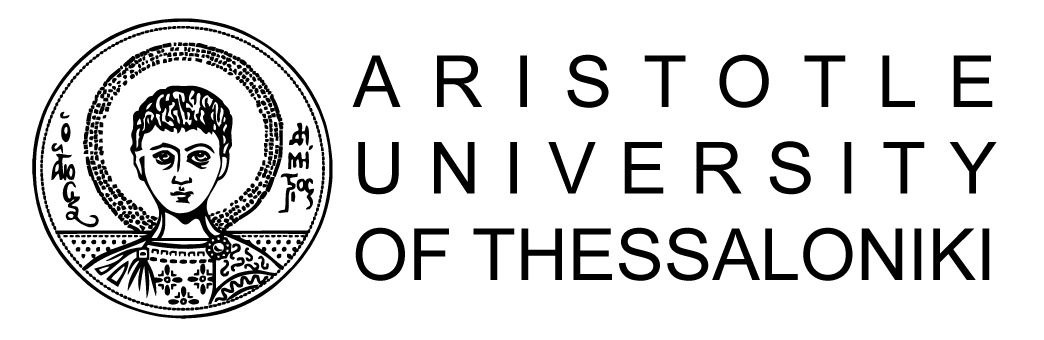
\includegraphics[width=0.8\textwidth]{banner-horizontal-black-en.png}\par % Image on top of title
\end{figure}
%\textcolor{black}{\large \bfseries Αριστοτέλειο Πανεπιστήμιο Θεσσαλονίκης\\}\par
\vspace{18pt}
\textcolor{black}{\Large \bfseries Department of Electrical\\ and Computer Engineering\\}\par
\vspace{1cm}
\vfill
\textcolor{black}{\Large \bfseries Group Project for the Game Theory Course}\par
\vspace{12pt}
\textcolor{black}{\large \bfseries Evolutionary Games Toolbox}\par

\vspace{0.5cm} % Adjust vertical spacing here
\vfill
\newcolumntype{L}{>{\raggedright\arraybackslash}X}%
\newcolumntype{R}{>{\raggedleft\arraybackslash}X}%
{\large
\def\arraystretch{1.3}
\begin{tabularx}{\textwidth}{ R|L }
\textbf{Group Number}                			 & 2           \\
\textbf{Delopoulos Emmanouil}      & entelopo@ece.auth.gr \\
\textbf{Vaporis Dimitrios}        & dvaporis@ece.auth.gr \\
\textbf{Voulkidis Vlasios}      & vlasiosv@ece.auth.gr \\
\textbf{Professor}           & Kehagias Athanasios\\
\end{tabularx}
}
\vspace{0.5cm}
\vfill
\textcolor{black}{\large \bfseries May 2025}\par
\end{titlepage}
\restoregeometry

\tableofcontents % Table of Contents

\clearpage
\section{Introduction}
\subsection{Description of the problem}
This is the report for the project of the course ``Game Theory'' of the Aristotle University of Thessaloniki. The subject of this project is the implementation and study of the Axelrod evolutionary tournament in the game "Prisoner's Dilemma." This name refers to a social dilemma, that is, any game of the form $\begin{bmatrix} R & S \\ T & P \end{bmatrix}$, where the following condition holds: $S < P < R < T$. Each player is given a choice, whether to cooperate or to defect. The payoff is calculated based on the player's move as well as the opponent's move; if both players cooperate, they each get R, if one cooperates and the other defects, the defector receives T and the cooperator receives S, otherwise if they both defect they both get rewarded P points. Paradoxically, a rational player may notice that no matter what the opponent plays, it is always better to defect, thus creating a Nash equilibrium (a game outcome that no player has motive to move away from) for two perfectly rational players in the ``Defect-Defect'' zone, making them both miss out on possible extra points, were they to cooperate. 

The repeated iteration of this game creates a match between strategies; multiple matches between strategies form a tournament, and the computation of a new population based on each strategy’s performance in the tournament constitutes the main focus of the study, an evolutionary tournament.

The project consists of four main functions, each of which performs a specific task that can be characterized by two features of the respective assumption: the nature of the simulation (theoretical or real) and the evolutionary dynamic (fitness or imitation). Each function is introduced individually, with an explanation of its operation and any assumptions made in each case. The first part of the project is largely based on the study by Mathieu et al. In fact, an effort was made to replicate the results as closely as possible to those presented in their 1999 paper.

For the study of the project, some concepts are crucial to understand. More specifically:
\begin{enumerate}
  \item A match is the base game played between two players, with a specified number of rounds (amount of times the players choose a move) which is unknown to the players.
  \item A strategy is a specific algorithm followed by a player in order to calculate their next move in a match.
  \item A population is the number of players following each strategy in a given tournament.
  \item A tournament consists of all possible matches between each pair of players (a player does not play against themselves though).
  \item An evolutionary game is the repetition of a tournament for a specified number of generations, where the population of each generation is calculated based on specified evolutionary dynamics.
\end{enumerate}

As mentioned above, the evolution dynamics studied in this project are the following:
\begin{enumerate}
  \item Fitness dynamics, where for each generation the number of players adopting each strategy is proportional to the performance (measured by a specific metric, in this case the total payoff in the tournament) of that strategy.
  \item Imitation dynamics, where after each generation a specified number of players adopt the best strategy (calculated either as an Individual or as a Total, more on that on a later chapter) of the previous generation.
\end{enumerate}

\subsection{Related Work}
The subject of the project was in large popularized by the famous Axelrod Tournament, where many famous game theorists were challenged to submit strategies for the Iterated Prisoner's Dilemma. The winning strategy ended up being the well-known Tit For Tat strategy, which, despite its simpleness, had many redeeming qualities; it was nice, meaning it was never the first to defect. It was retaliatory, meaning it was ready to counter attack if the opponent defects. It was also forgiving, meaning it did not hold a grudge too long; if an opponent defected but repented, Tit For Tat forgave them and continued to cooperate. Lastly, it was clear; it is not difficult for the opponent to understand the intentions of the strategy, thus making it more likely that cooperation occurs.

Since 1980, when the tournament was held, a large number of studies have been published on the matter, a lot of which have focused on the evolutionary aspect of the tournament, trying to mimic the actual evolution of species in the animal kingdom, as well as the birth of cooperation between humans. One such paper was published in 1999 by Philippe Mathieu, Bruno Beaufils and Jean-Paul Delahaye with title ``Studies on Dynamics in the Classical Iterated Prisoner's Dilemma with Few Strategies''. In this specific paper, the evolutionary dynamics analyzed were Fitness Dynamics and the results aimed to showcase the different possible forms of dynamics that can occur and which aspects of the simulation they may depend on. As mentioned previously, the first part of this project is based exactly on that paper, aiming to recreate the results presented by Mathieu et al, as well as modifying the dynamics slightly to notice any differences in the resulting dynamics.
\clearpage
\section{Quickstart}

TO DO: Add a quick start text as instructed.
\section{Fitness Dynamics}

The first evolutionary dynamics to be analyzed (and the one studied by Mathieu et al.) are the \textbf{Fitness Dynamics}, according to which each strategy in the simulation is assigned a score, which is then used to calculate the population distribution for the next generation. The approach followed in both functions that use fitness is that of Mathieu et al., where the fitness of each strategy is calculated as follows:

Suppose the population consists of 3 strategies, A, B, and C. Based on the game matrix $B$, the number of rounds per match $T$, and, of course, the strategies that face each other in each case, the payoffs for each of the two strategies are calculated and stored as, for example, $V(A|B)$, the payoff of strategy A when it faces strategy B. Then, the score for each player using a given strategy (and thus, essentially, the score of the strategy itself) is calculated as, for example, for strategy A:

\[
g_n(A) = W_n(A)V(A|A) + W_n(B)V(A|B) + W_n(C)V(A|C) - V(A|A)
\]

where $W_n(A), W_n(B), W_n(C)$ are the population sizes of each strategy in generation $n$. (Note that the payoff for playing against one’s own strategy is subtracted once, because it is assumed that individuals do not play against themselves.)

Finally, the total tournament score is calculated as:

\[
t(n) = W_n(A)g_n(A) + W_n(B)g_n(B) + W_n(C)g_n(C)
\]

and the population in generation $n+1$ for strategy A becomes:

\[
W_{n+1}(A) = \frac{\Pi W_n(A)g_n(A)}{t(n)}
\]

It should be emphasized that this logic is applied due to the fully deterministic nature of the implemented strategies. If there were strategies with random elements, the theoretical calculation of the outcome of each match would be impossible, and one would instead need to compute some expected value---something that falls outside the scope of this study.
\subsection{The function TourSimFit}
The first function implemented is \texttt{[POP, BST, FIT] = TourSimFit(B, Strategies, POP0, T, J, compensation)}, where $B$ is the payoff matrix of the game, \texttt{Strategies} is an array of strings with the names of the strategies participating in the simulation, \texttt{POP0} is the initial population, $T$ is the number of rounds in each match, and $J$ is the number of generations of the evolutionary tournament. Additionally, \texttt{compensation} is an optional boolean argument (the function can be called without including it), whose function is described below. The function returns the following:

\begin{itemize}
    \item \texttt{POP}: a matrix with the population of each strategy per generation,
    \item \texttt{BST}: a matrix indicating the best strategies in each round (0 if not among the best, 1 if among the best — ties are counted),
    \item \texttt{FIT}: a matrix with the fitness scores of each strategy for each generation.
\end{itemize}

The logic of the function follows what was presented earlier, but an additional mechanism is added during the computation of the next generation’s populations to avoid decimal values and ensure that the population for each strategy in each generation remains an integer. The logic works as follows:

The initial result of the population computations is taken as the \texttt{floor} of the decimal values. Then, any deficit that arises from applying the floor function is computed, and one new player at a time is randomly assigned to some strategy, until the deficit is eliminated. A check is also performed to ensure that the strategy does not already have a population of zero, to avoid its "revival." In this way, the total player population remains constant throughout the simulation, as is assumed by Mathieu et al.

This choice is deliberate. Cases were tested in which each player was assigned to the strategy whose calculated population was closest to the next integer (e.g., if a strategy had an initial computed population of 199.8, it would be rounded to 200), as well as the opposite case, where players were assigned to the strategy furthest from the next integer. These algorithms showed some undesirable behaviors, such as maintaining a very small number of players in certain strategies (e.g., a strategy remaining stuck at population 2 because the next generation’s computed population is 1.8, or 1.1 respectively). By preserving this random element, the simulation results do not differ significantly from those without randomness, while the method guarantees that weaker strategies are completely eliminated over time.

However, observing the deviation of this implementation from the results in the paper, we added the following adjustment: an extra boolean argument in the function \texttt{TourSimFit}, named \texttt{compensation} with default value \texttt{false}, which performs the functionality described below. With value \texttt{false}, it returns results using only simple rounding to the nearest lower integer (floor rounding), which we believe is also the method used in the paper. In this case, the population per generation is not necessarily constant, but the deviation does not increase additively — perhaps just 1 or 2 individuals are lost in some generations due to rounding down. With value \texttt{true}, it returns results according to the player-reassignment logic described earlier. Below the main loop for the tournament simulation, including the possible compensation of the deficiency in the population, is presented with pseudocode.

\begin{algorithm}
\caption{TourSimFit Simulation}
\begin{algorithmic}[1]
\FOR{$i = 1$ to $J$}
    \FOR{$j = 1$ to $N_{\text{strat}}$}
        \STATE $FIT[i][j] \gets 0$
        \FOR{$k = 1$ to $N_{\text{strat}}$}
            \STATE $FIT[i][j] \gets FIT[i][j] + \text{payoff}[j][k] \cdot POP[i][k]$
        \ENDFOR
        \STATE $FIT[i][j] \gets FIT[i][j] - \text{payoff}[j][j]$
    \ENDFOR

    \STATE $maxVal \gets \max(FIT[i][:])$
    \STATE $allMaxIndices \gets \{j \mid FIT[i][j] = maxVal\}$
    \FORALL{$j \in allMaxIndices$}
        \STATE $BST[i][j] \gets 1$
    \ENDFOR

    \STATE $total\_each \gets POP[i][:] \cdot FIT[i][:]$ \COMMENT{Element-wise multiplication}
    \STATE $total \gets \sum total\_each$

    \FOR{$j = 1$ to $N_{\text{strat}}$}
        \STATE $POP[i+1][j] \gets \left\lfloor POP[i][j] \cdot \dfrac{FIT[i][j]}{total} \cdot N \right\rfloor$
    \ENDFOR

    \IF{$compensation$ is \textbf{true}}
        \STATE $N_{new} \gets \sum POP[i+1][:]$
        \STATE $deficiency \gets N - N_{new}$
        \WHILE{$deficiency > 0$}
            \STATE $k \gets \text{random integer in } [1, N_{\text{strat}}]$
            \IF{$POP[i][k] = 0$}
                \STATE \textbf{continue}
            \ENDIF
            \STATE $POP[i+1][k] \gets POP[i+1][k] + 1$
            \STATE $deficiency \gets deficiency - 1$
        \ENDWHILE
    \ENDIF
\ENDFOR
\end{algorithmic}
\end{algorithm}

In the simulations that follow, a comparison is also presented between these two methods and the results of the function \texttt{TourTheFit}, which is described below. Including the results from the paper was deemed unnecessary.


\subsection{The function TourTheFit}
The second function implemented is [POP,BST,FIT]\- =\- TourTheFit\- (B,\- Strategies,\- POP0,\- T,\- J), with arguments and outputs entirely identical to those of the previous one. The only substantial difference lies in the fact that now, due to the theoretical nature of the simulation, the part of the code responsible for maintaining integer values in the population is omitted, since decimal numbers are allowed, as the population does not actually consist of individual players. Below, the main loop of the evolutionary tournament is presented via pseudocode.

\begin{algorithm}
\caption{TourTheFit Simulation}
\begin{algorithmic}[1]
\FOR{$i = 1$ to $J$}
    \FOR{$j = 1$ to $N_{\text{strat}}$}
        \STATE $FIT[i][j] \gets 0$
        \FOR{$k = 1$ to $N_{\text{strat}}$}
            \STATE $FIT[i][j] \gets FIT[i][j] + \text{payoff}[j][k] \cdot POP[i][k]$
        \ENDFOR
        \STATE $FIT[i][j] \gets FIT[i][j] - \text{payoff}[j][j]$
    \ENDFOR

    \STATE $maxVal \gets \max(FIT[i][:])$
    \STATE $allMaxIndices \gets \{j \mid FIT[i][j] = maxVal\}$
    \FORALL{$j \in allMaxIndices$}
        \STATE $BST[i][j] \gets 1$
    \ENDFOR

    \STATE $total\_each \gets POP[i][:] \cdot FIT[i][:]$ \COMMENT{Element-wise multiplication}
    \STATE $total \gets \sum total\_each$

    \FOR{$j = 1$ to $N_{\text{strat}}$}
        \STATE $POP[i+1][j] \gets POP[i][j] \cdot \dfrac{FIT[i][j]}{total} \cdot N$
    \ENDFOR
\ENDFOR
\end{algorithmic}
\end{algorithm}

\subsection{Simulations - Examples}
From this point on, the simulations of the fitness dynamics are presented, using the functions discussed above. Each plot presented is created by the corresponding example referenced in the text, contained in the Examples folder of the GitHub repository. For a more detailed description of each call and the parameters used in each example, please refer to the Documentation.pdf file contained in the Documentation folder of the repository, as well as the actual source code of each example. Along with the plots created by the functions described, the plots of the original 1999 paper by Mathieu et al are presented, so as to allow direct comparison and discussion of every example. 
\subsubsection{1st Simulation - Defectors may be strong}
Already from the first simulation (Figure~\ref{fig:Defectors may be strong}), an interesting result emerges. The purpose of this simulation is to demonstrate that, in specific sets of strategies and favorable initial population values, defecting strategies such as \texttt{per\_ddc} are capable of dominating. However, the theoretical analysis of the scenario studied in the paper does not present exactly the same picture. This is due to the fact that the population of \texttt{soft\_majo} in the simulation cases completely disappears around the 20th generation, whereas in the theoretical case, this does not occur. Thus, after a few generations and a relative decrease in the population of \texttt{per\_ddc}, the strategy \texttt{soft\_majo} returns and the strategy \texttt{Alternator} develops, which is essentially the perfect opponent of \texttt{soft\_majo}, as it defects exactly as much as necessary to keep \texttt{soft\_majo} cooperating. After a certain point, of course, both of these populations begin to decline again, while the population of \texttt{per\_ddc} increases, which leads us to suspect that this example theoretically results in oscillation. In the simulations, however---in both the \texttt{compensation} case and the one without it---the results are very similar to those in the paper: the slight variation in the \texttt{compensation} case is due to the stochastic element, which makes the curve appear less smooth than in the case without \texttt{compensation}. Run example01 of the Examples folder (after reading Quickstart guide) to recreate the figure.

	\begin{figure}[h]
		\centering
		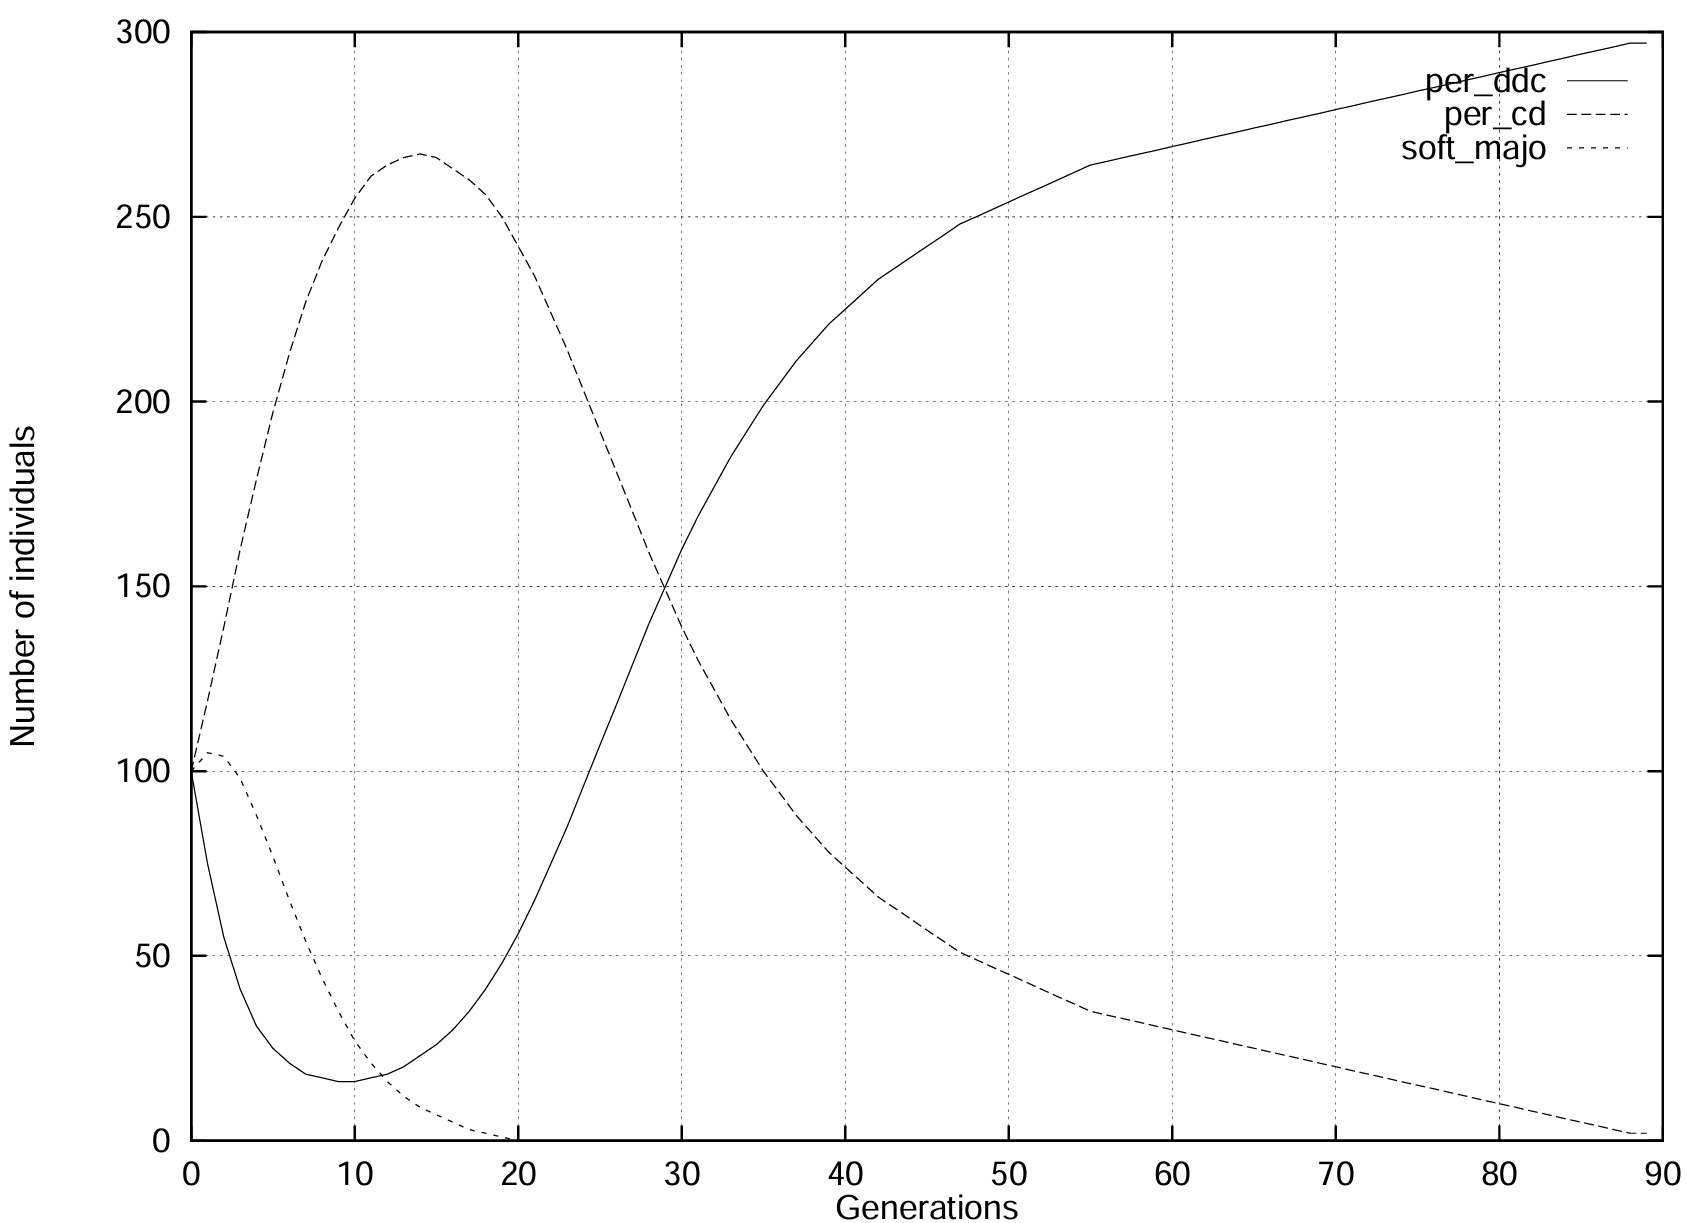
\includegraphics[width=0.7\textwidth]{RefPaperFigures/fig1.jpeg}\par\vspace{0.5em}
		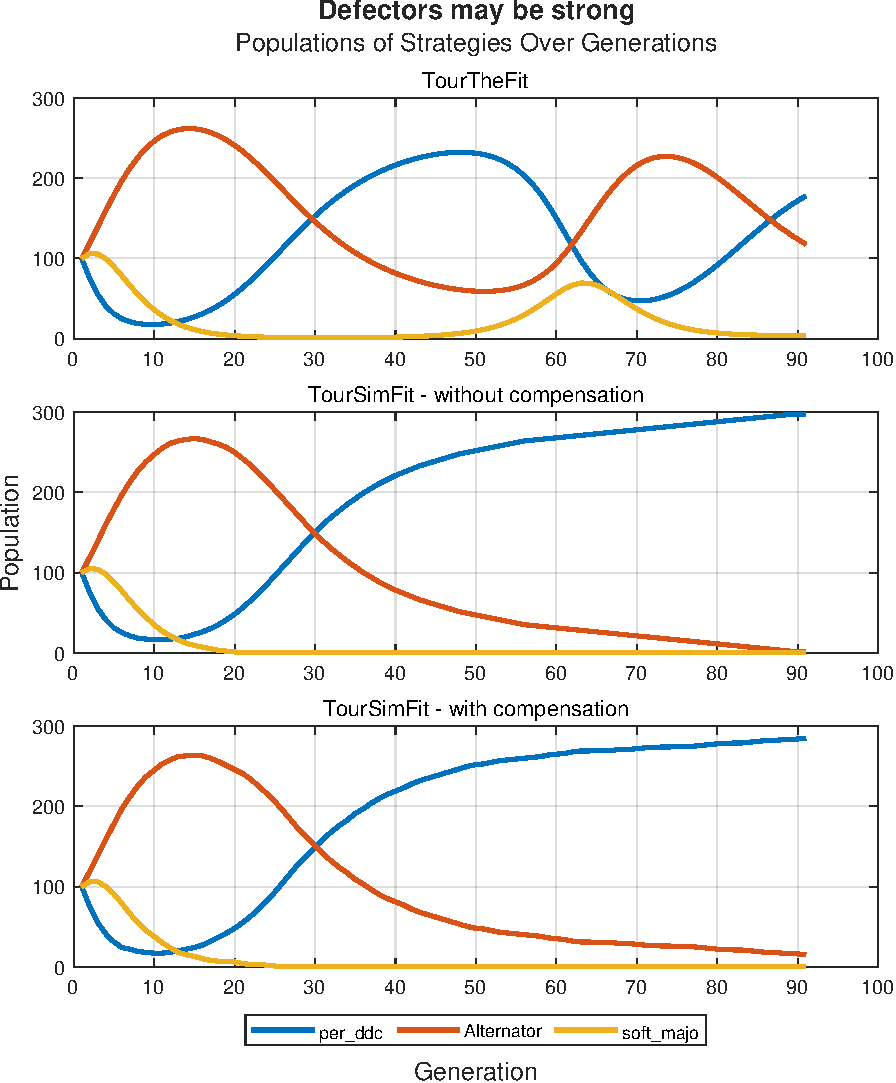
\includegraphics[width=0.7\textwidth]{Defectors may be strong.pdf}
	    \caption{1st Simulation - Defectors may be strong}
	    \label{fig:Defectors may be strong}
	\end{figure}
\subsubsection{2nd Simulation - Monotonous Convergence}
From now on, the results are presented for the simulations used by Mathieu et al. to classify the graphs into 5 categories, the first of which (Figure~\ref{fig:Monotonous Convergence}) is the monotonous convergence of populations. This is the most common form that emerges, as the oscillations presented below are quite sensitive to initial conditions. The results of both the theoretical analysis and the two simulations are identical to those of Mathieu et al., with the only difference being a slightly different final population in the case of \texttt{compensation}, which is again due to the stochastic element. However, the ranking of the strategies remains the same. Run example02 of the Examples folder (after reading Quickstart guide) to recreate the figure.

	\begin{figure}[h]
	    \centering
		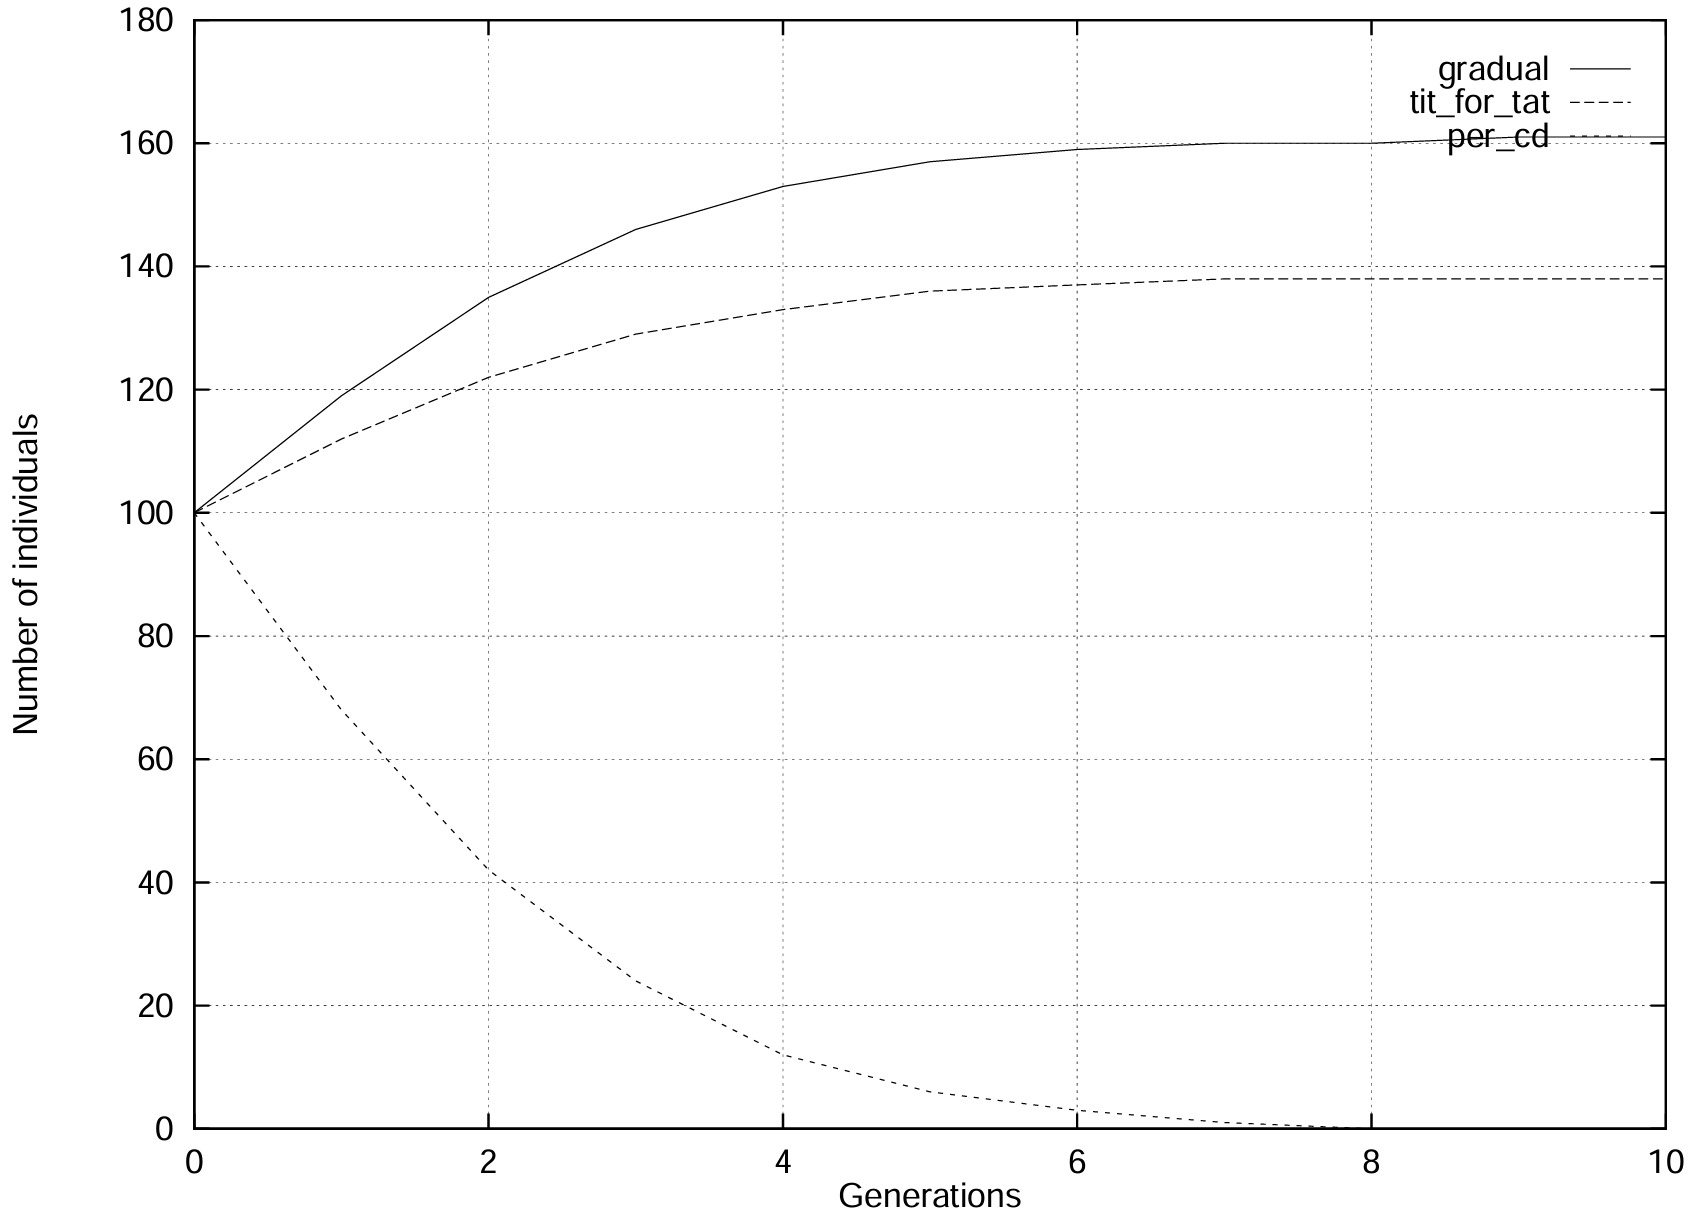
\includegraphics[width=0.7\textwidth]{RefPaperFigures/fig2.jpeg}\par\vspace{0.5em}
	    \includegraphics[width=0.7\textwidth]{Monotonous Convergence.pdf}
	    \caption{2nd Simulation - Monotonous Convergence}
	    \label{fig:Monotonous Convergence}
	\end{figure}
\subsubsection{3rd Simulation - Attenuated Oscillatory movements}
The next category of results from the paper is the diminishing oscillations of populations (Figure~\ref{fig:Attenuated oscillatory movements}). The results in this case are identical to those of Mathieu et al. for all three cases presented. The initial populations in this particular case are quite large, so the one or two players that randomly oppose in the \texttt{compensation} scenario do not significantly affect the trajectory of the function. Run example03 of the Examples folder (after reading Quickstart guide) to recreate the figure.

	\begin{figure}[h]
	    \centering
		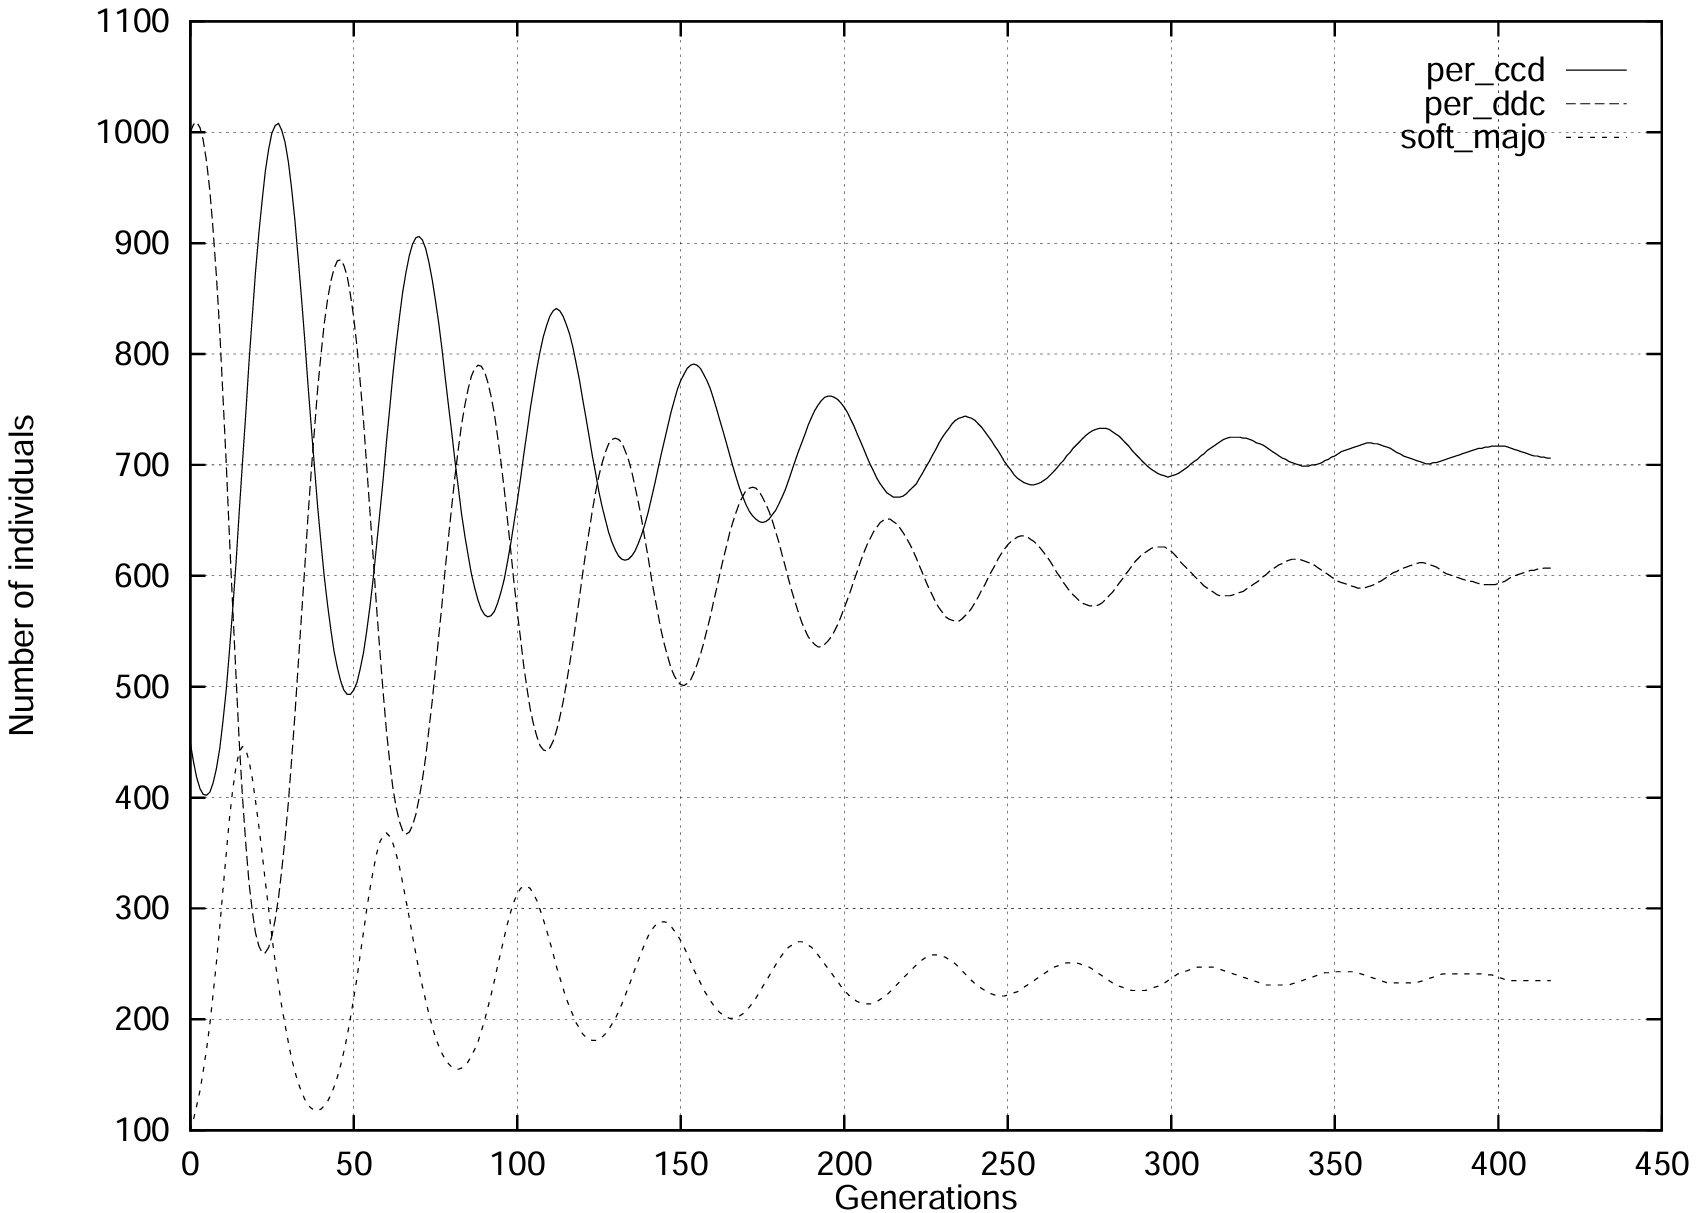
\includegraphics[width=0.7\textwidth]{RefPaperFigures/fig3.jpeg}\par\vspace{0.5em}
	    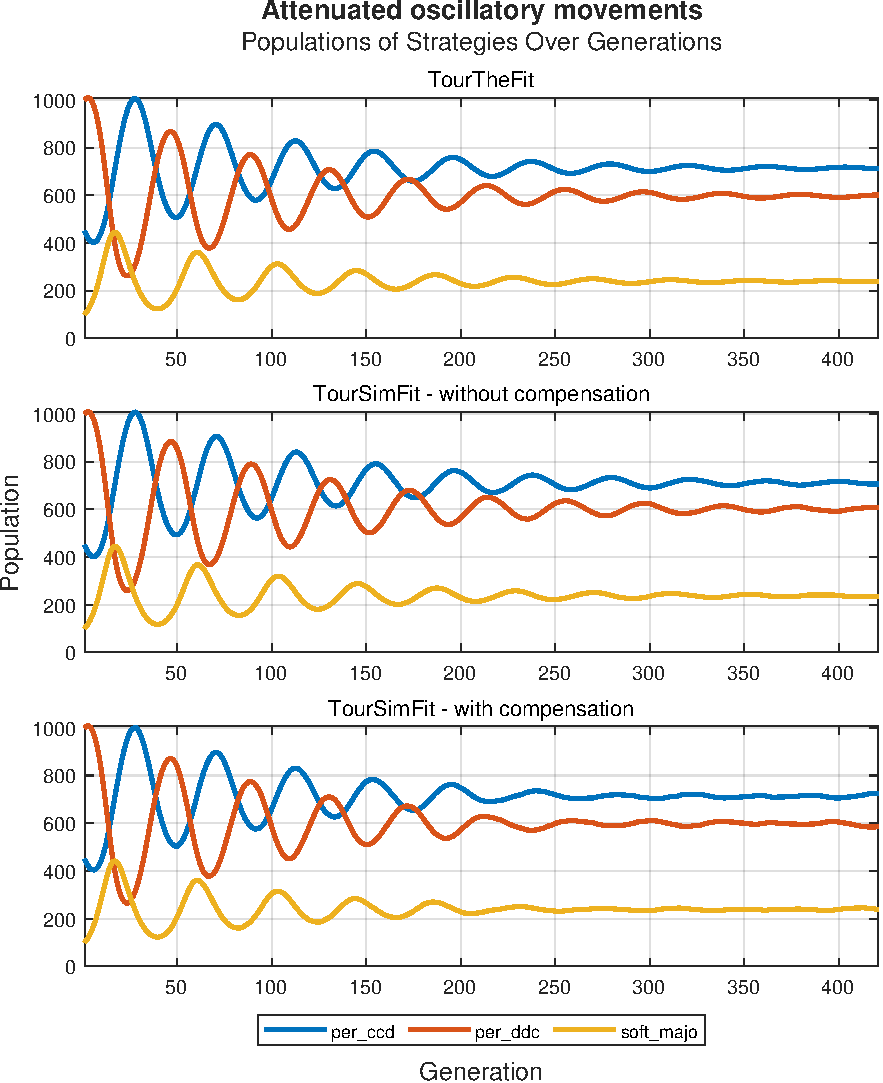
\includegraphics[width=0.7\textwidth]{Attenuated oscillatory movements.pdf}
	    \caption{3rd Simulation - Attenuated oscillatory movements}
	    \label{fig:Attenuated oscillatory movements}
	\end{figure}
\subsubsection{4th Simulation - Periodic movements}
The third case is the appearance of periodic movements/oscillations (Figure~\ref{fig:Periodic movements}), without an increase or decrease in the amplitude of the oscillations. This behavior generally appears when there are three strategies with a "rock-paper-scissors" logic: the 1st "beats" the 2nd, which "beats" the 3rd, which in turn "beats" the 1st. In this particular case, \texttt{per\_ccd} beats \texttt{soft\_majo}, which beats \texttt{per\_ddc}, which beats \texttt{per\_ccd}. With appropriate initial populations, the following results are observed. The theoretical analysis shows that the oscillation actually fades — it is a diminishing oscillation as before. This is due to the fact that in discrete cases, such as these simulations, it becomes certain through suitable choices that the system will return to a previous state, and thus repetition/oscillation will occur. However, in the theoretical analysis, this does not happen (due to the "infinity" of states because of decimal numerics), and thus the oscillation is damped. The \texttt{TourSimFit} function without \texttt{compensation} again yields results identical to those of Mathieu et al., while the case with \texttt{compensation}, although visually less appealing, also captures the oscillation, even with noticeable noise due to randomness (the amplitudes of the oscillations are small, so even the addition of one or two extra players has a noticeable effect). Run example04 of the Examples folder (after reading Quickstart guide) to recreate the figure.

	\begin{figure}[h]
	    \centering
		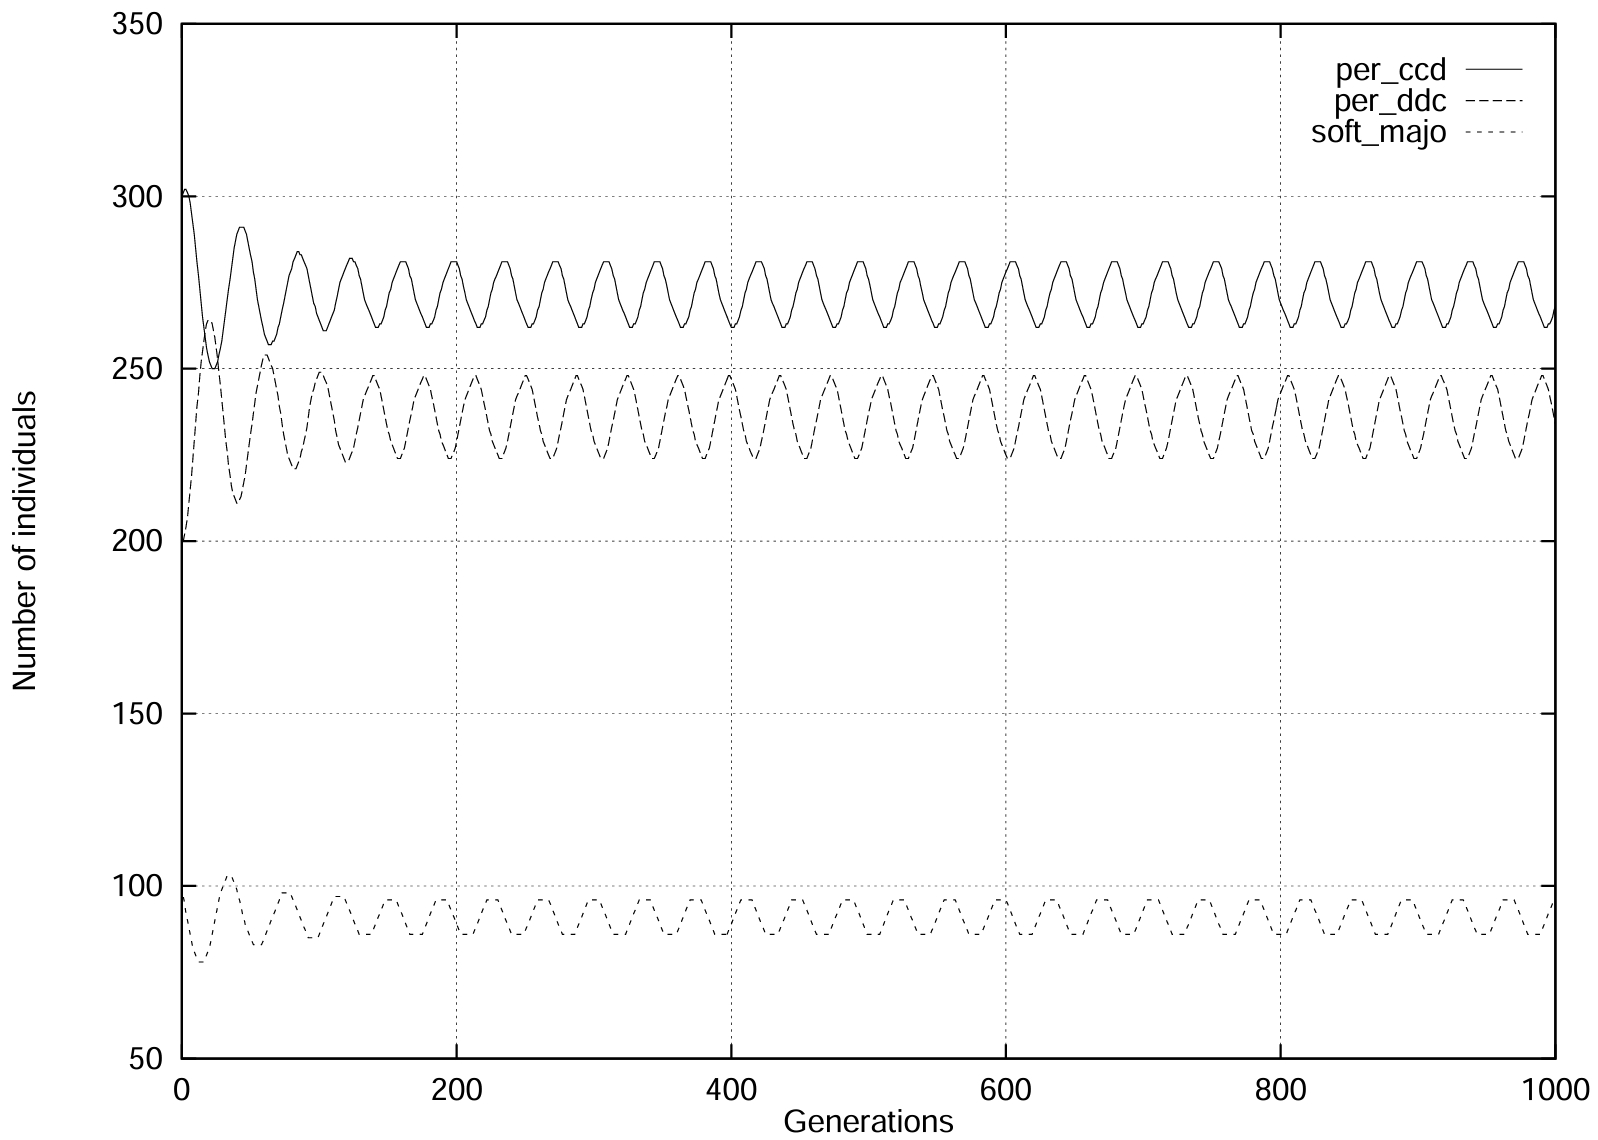
\includegraphics[width=0.7\textwidth]{RefPaperFigures/fig4.jpeg}\par\vspace{0.5em}
	    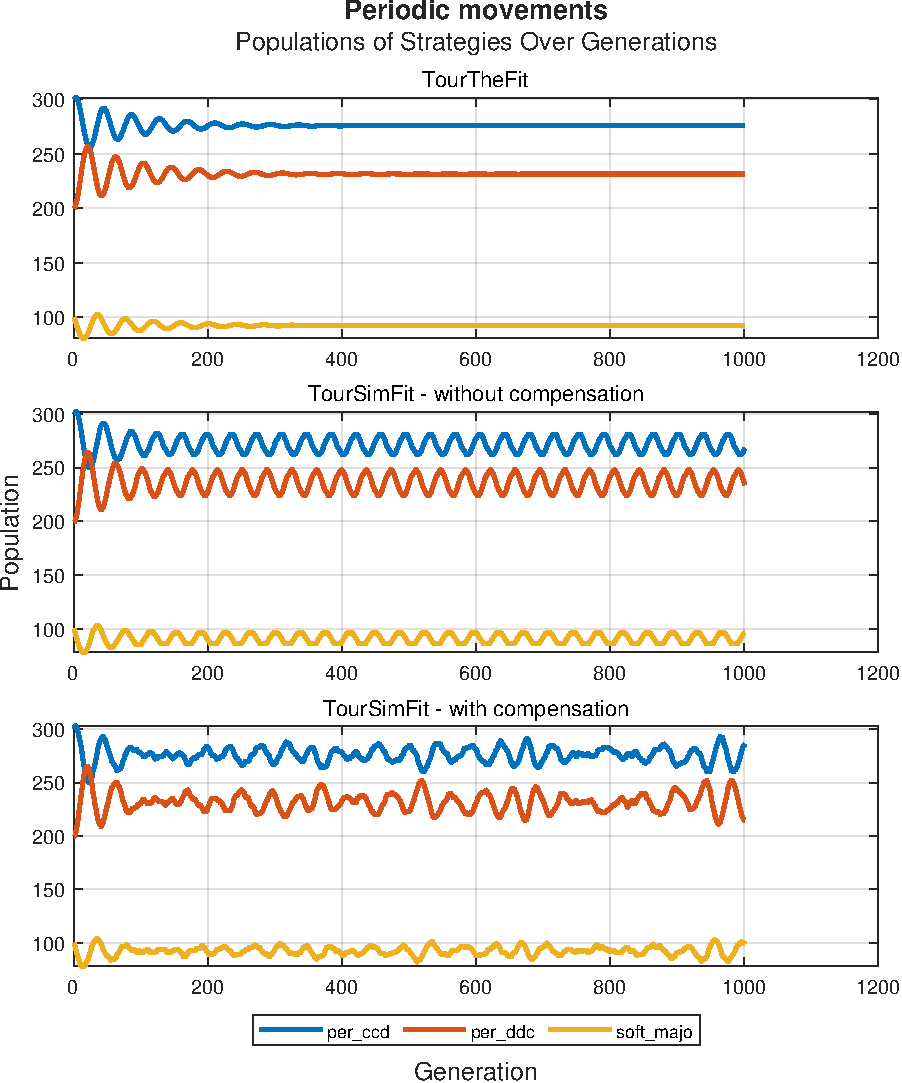
\includegraphics[width=0.7\textwidth]{Periodic movements.pdf}
	    \caption{4th Simulation - Periodic movements}
	    \label{fig:Periodic movements}
	\end{figure}
\subsubsection{5th Simulation - Increasing oscillations}
One of the most unexpected cases is that of increasing oscillations (Figure~\ref{fig:Increasing oscillations}). With an appropriate choice of the payoff matrix, strategies, and initial populations, this phenomenon can be observed. The population was initially tested as is, but the results were not satisfactory. Therefore, the payoff matrix was changed to 
\[
B = \begin{bmatrix} 3 & 0 \\ 4.72 & 1 \end{bmatrix}
\]
(using trial and error, knowing the general direction in which the matrix needed to be changed towards), and eventually, a result very similar to that of the paper was observed in the case of \texttt{TourSimFit} without \texttt{compensation}. However, for the same value of \( B \) and the cases of \texttt{TourTheFit} and \texttt{TourSimFit} with \texttt{compensation}, slightly diminishing oscillations are observed, revealing two truths about the cases of increasing oscillations. First, they arise from populations capable of exhibiting normal oscillations, with a suitable modification of the payoff matrix. Second, they are particularly sensitive cases that collapse back into normal or diminishing oscillations with even a slight modification of the dynamics (such as the logic of \texttt{compensation}). It is quite possible that for an appropriate choice of \( B \), the cases of \texttt{TourTheFit} and \texttt{TourSimFit} with \texttt{compensation} could also transform into increasing oscillations, but it was considered more important for this work to present this divergence in the results. Run example05 of the Examples folder (after reading Quickstart guide) to recreate the figure.

	\begin{figure}[h]
	    \centering
		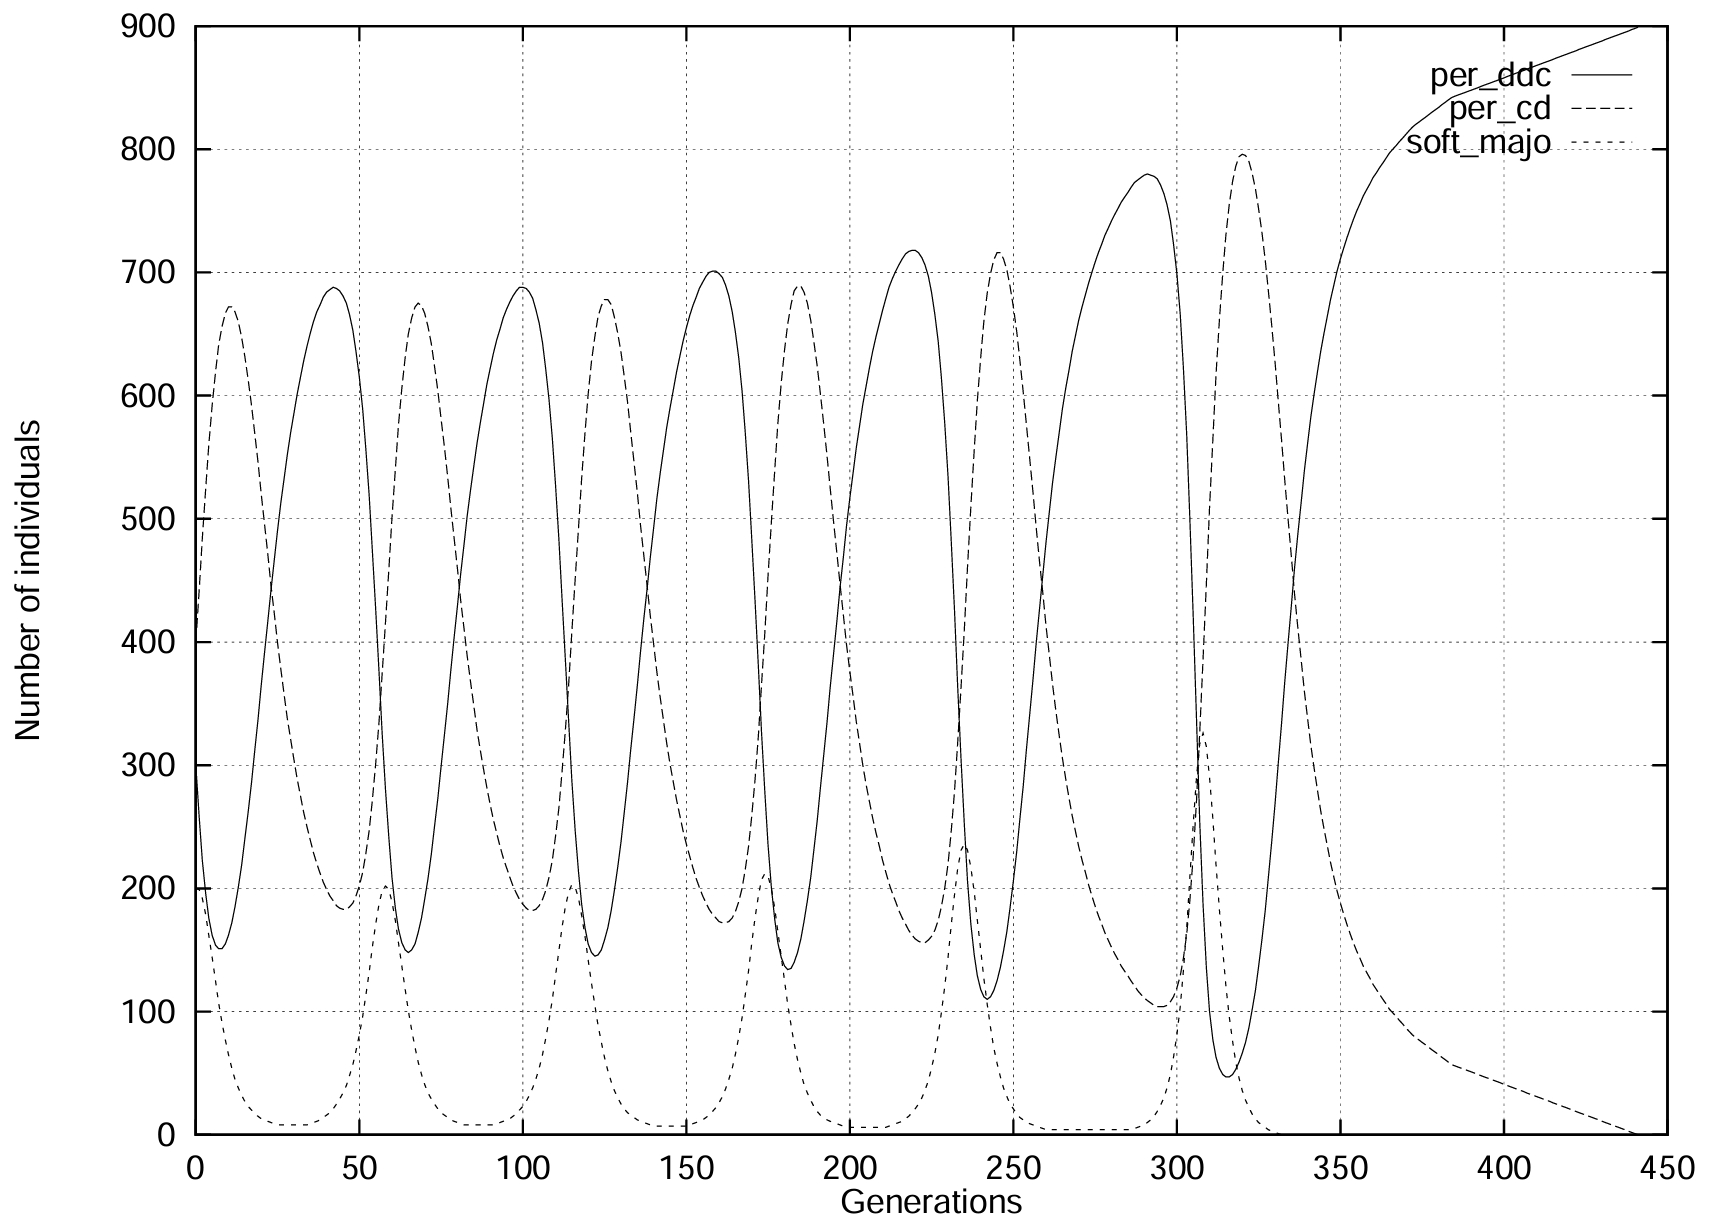
\includegraphics[width=0.7\textwidth]{RefPaperFigures/fig5.jpeg}\par\vspace{0.5em}
	    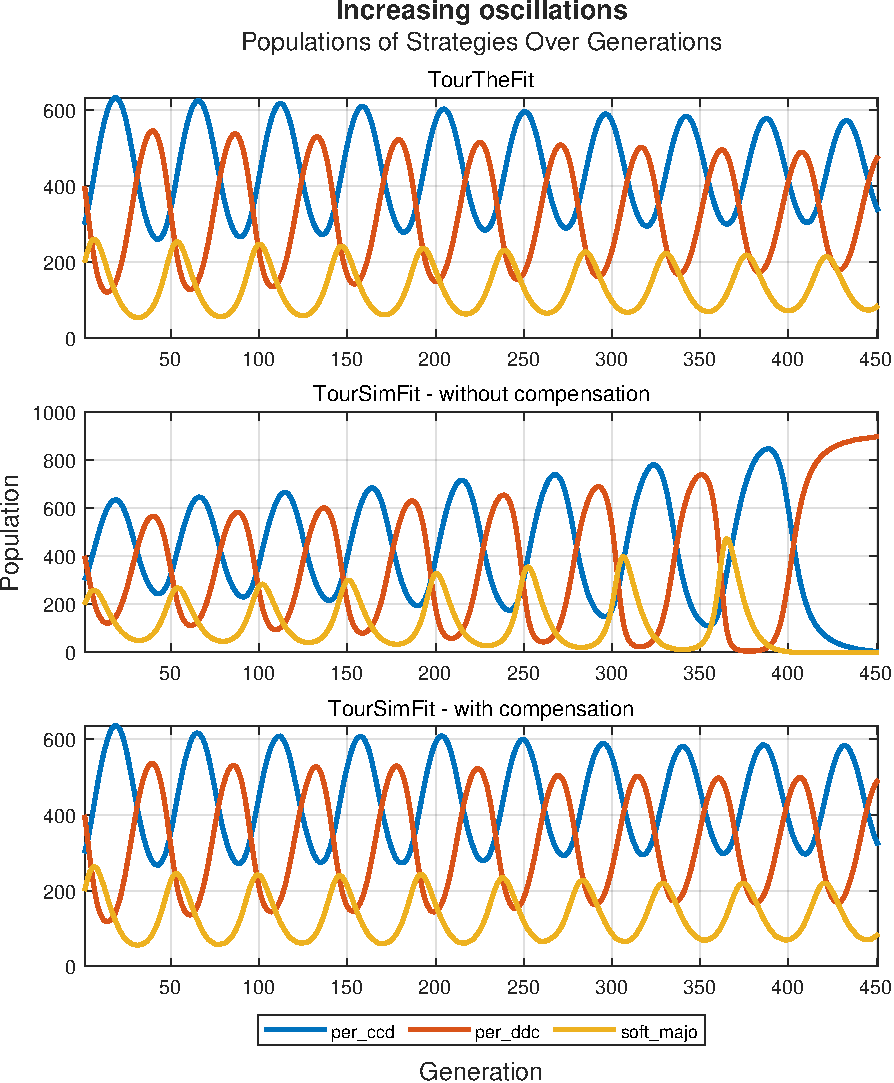
\includegraphics[width=0.7\textwidth]{Increasing oscillations.pdf}
	    \caption{5th Simulation - Increasing oscillations}
	    \label{fig:Increasing oscillations}
	\end{figure}
\subsubsection{6th Simulation - Chaos/Disordered oscillations}
The last case presented in the paper is that of disordered oscillations (Figure~\ref{fig:Disordered oscillations}). The authors of the paper rightly hesitate to characterize it as a truly chaotic case because, due to the discrete nature of the simulation, any such behavior after a sufficient number of generations either reaches equilibrium or simply repeats. However, the results of this particular simulation appear quite chaotic to the eye. Again, the case of \texttt{TourSimFit} without \texttt{compensation} fully matches the results of the paper. In contrast, due to the sensitivity of the phenomenon, the cases of the theoretical analysis and the actual simulation with \texttt{compensation} differ significantly, as they do not exhibit the chaotic behavior around generation 140 as in the case of the paper. Nevertheless, they predict the survival of the \texttt{per\_ccccd} and \texttt{Prober} strategies, as well as the values toward which the populations in the \texttt{TourSimFit} case without simulation seem to tend. Run example06 of the Examples folder (after reading Quickstart guide) to recreate the figure.

	\begin{figure}[h]
	    \centering
		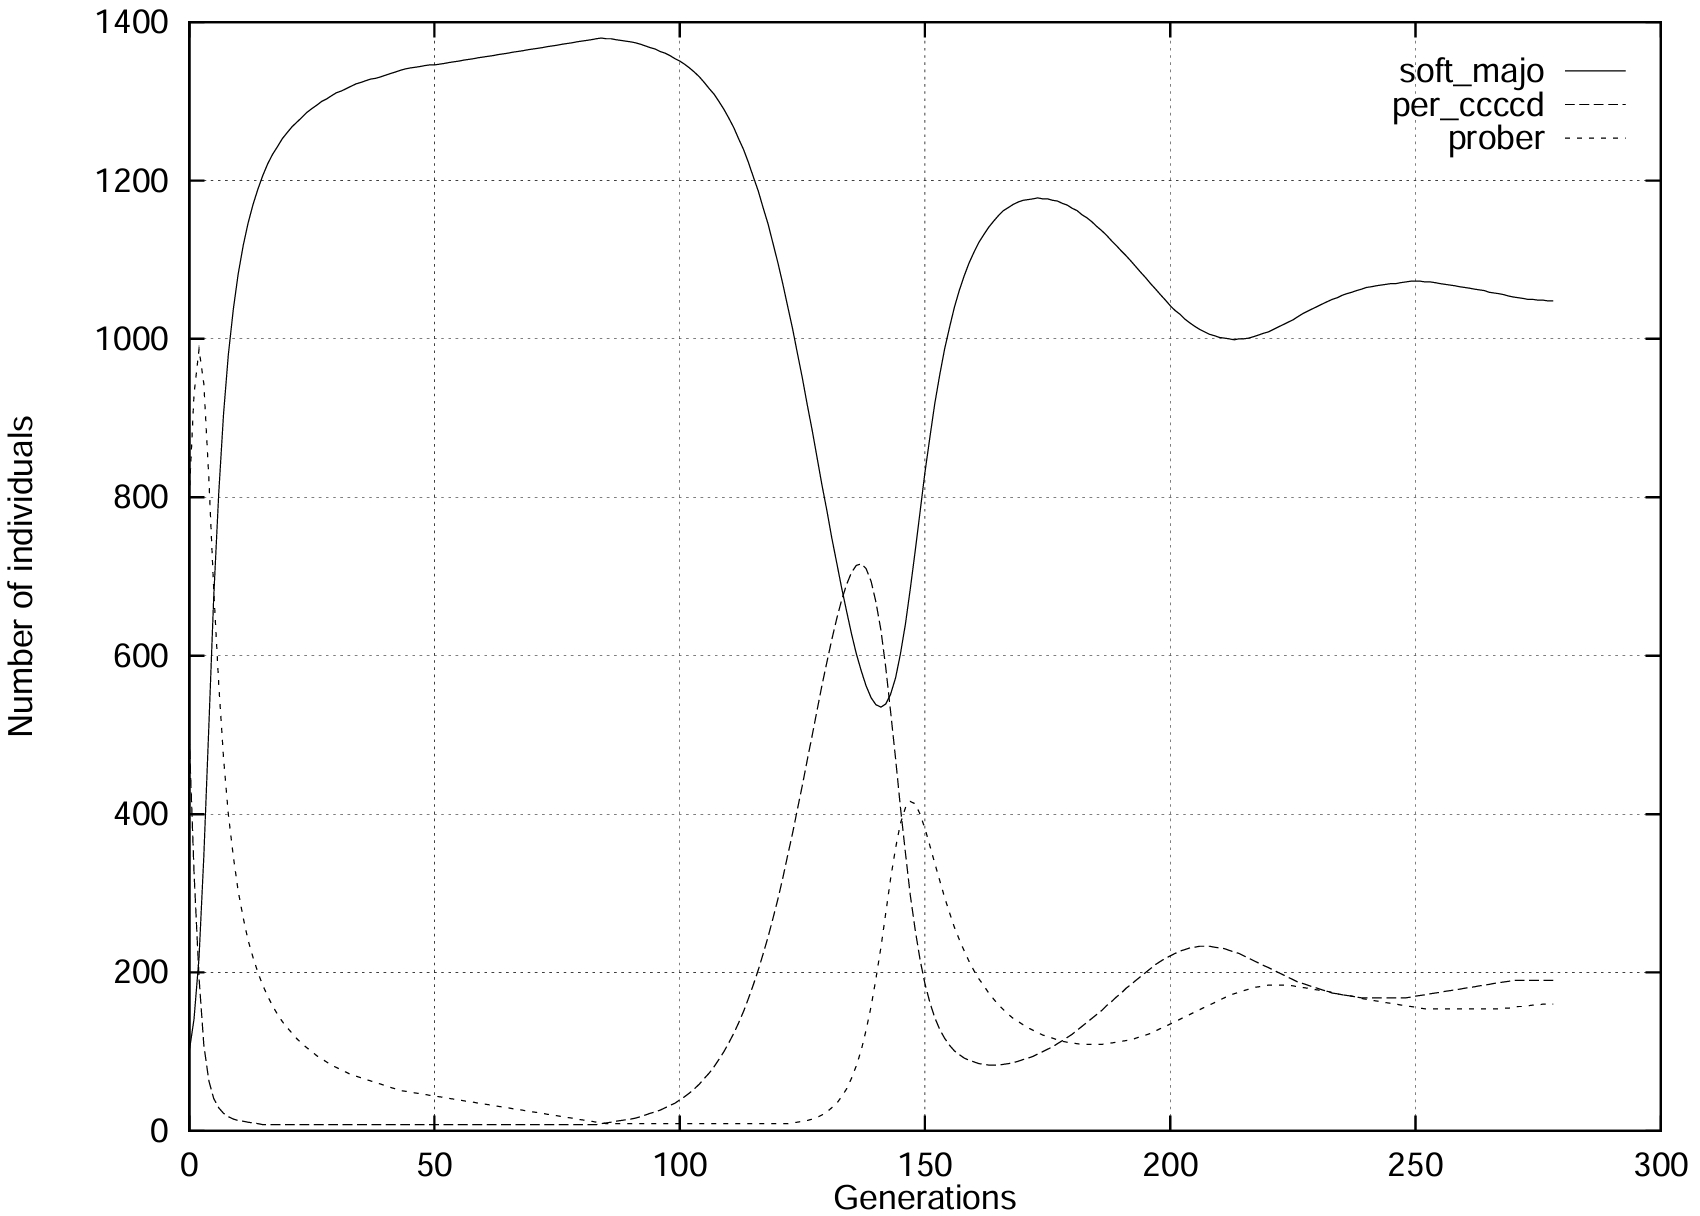
\includegraphics[width=0.7\textwidth]{RefPaperFigures/fig6.jpeg}\par\vspace{0.5em}
	    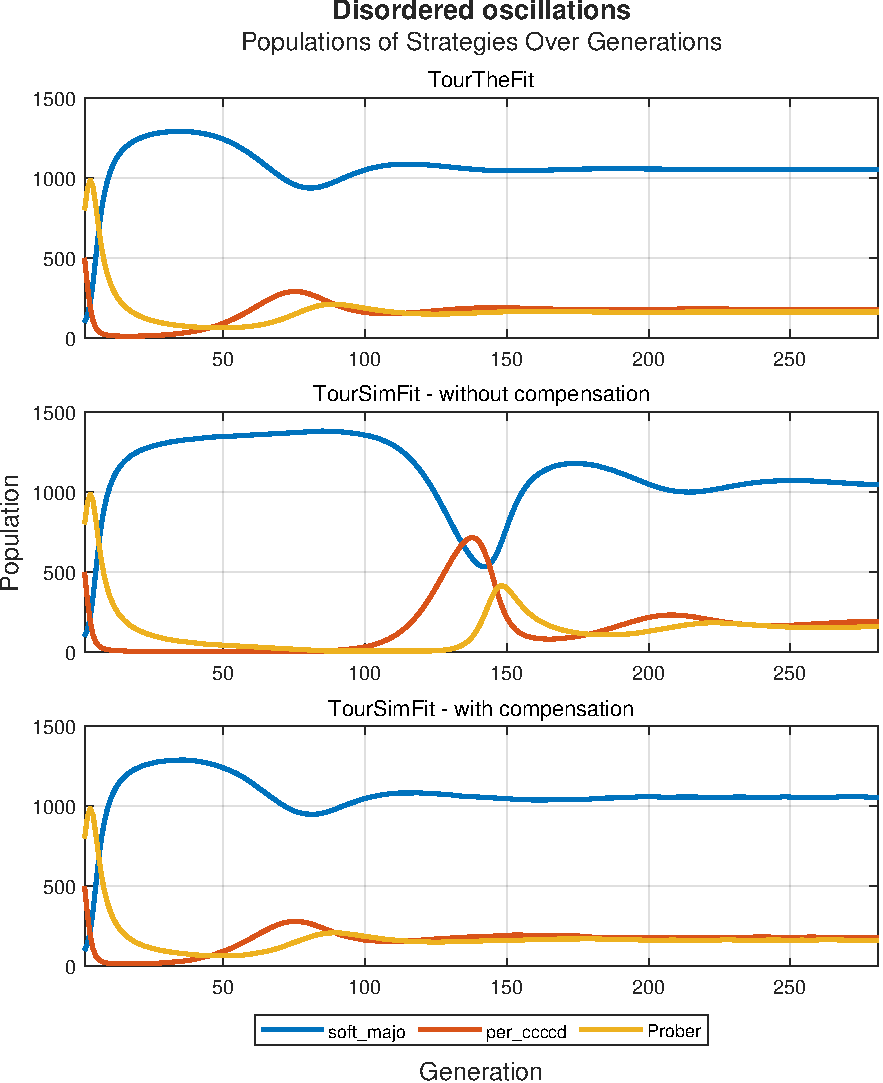
\includegraphics[width=0.7\textwidth]{Disordered oscillations.pdf}
	    \caption{6th Simulation - Disordered oscillations}
	    \label{fig:Disordered oscillations}
	\end{figure}

\subsubsection{7th Simulation - Sensitivity of dynamics to population's size - First Simulation}
	\begin{figure}[h]
	    \centering
		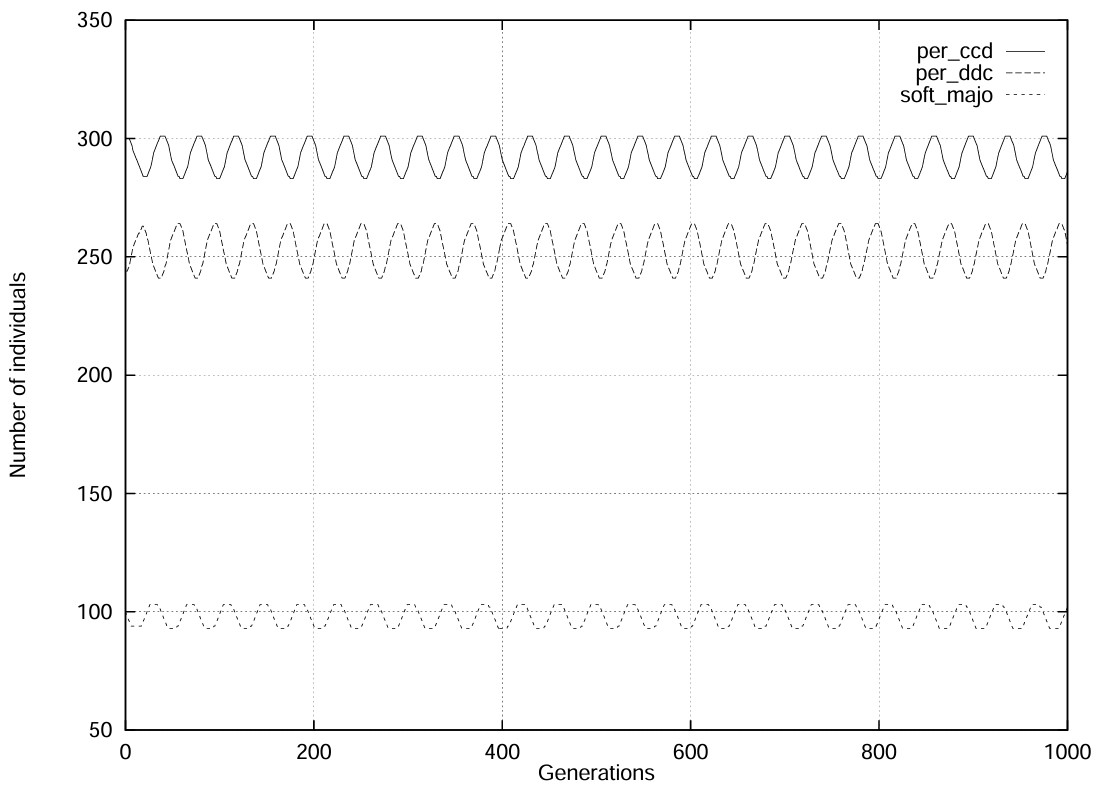
\includegraphics[width=0.7\textwidth]{RefPaperFigures/fig7a.jpeg}\par\vspace{0.5em}
	    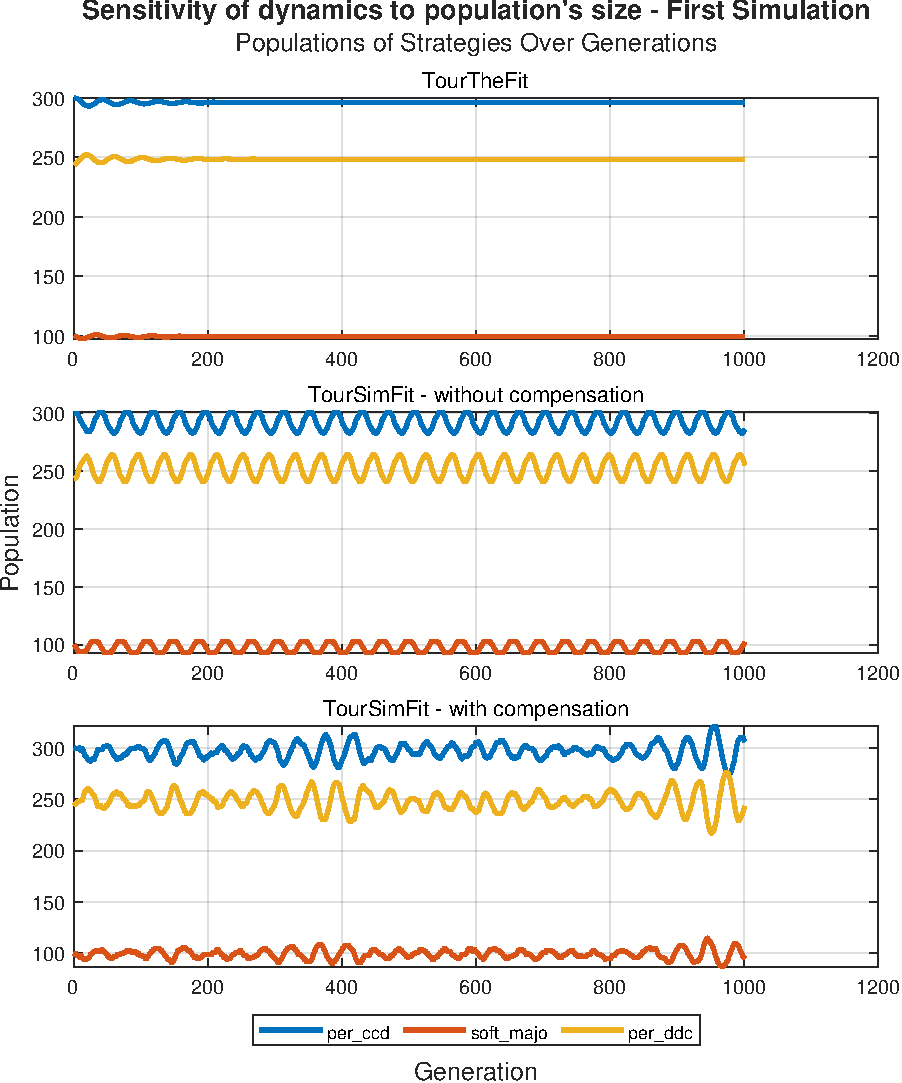
\includegraphics[width=0.7\textwidth]{Sensitivity of dynamics to population's size - First Simulation.pdf}
	    \caption{7th Simulation - Sensitivity of dynamics to population's size - First Simulation}
	    \label{fig:Sensitivity of dynamics to population's size - First Simulation}
	\end{figure}
\subsubsection{8th Simulation - Sensitivity of dynamics to population's size - Second Simulation}
	\begin{figure}[h]
	    \centering
		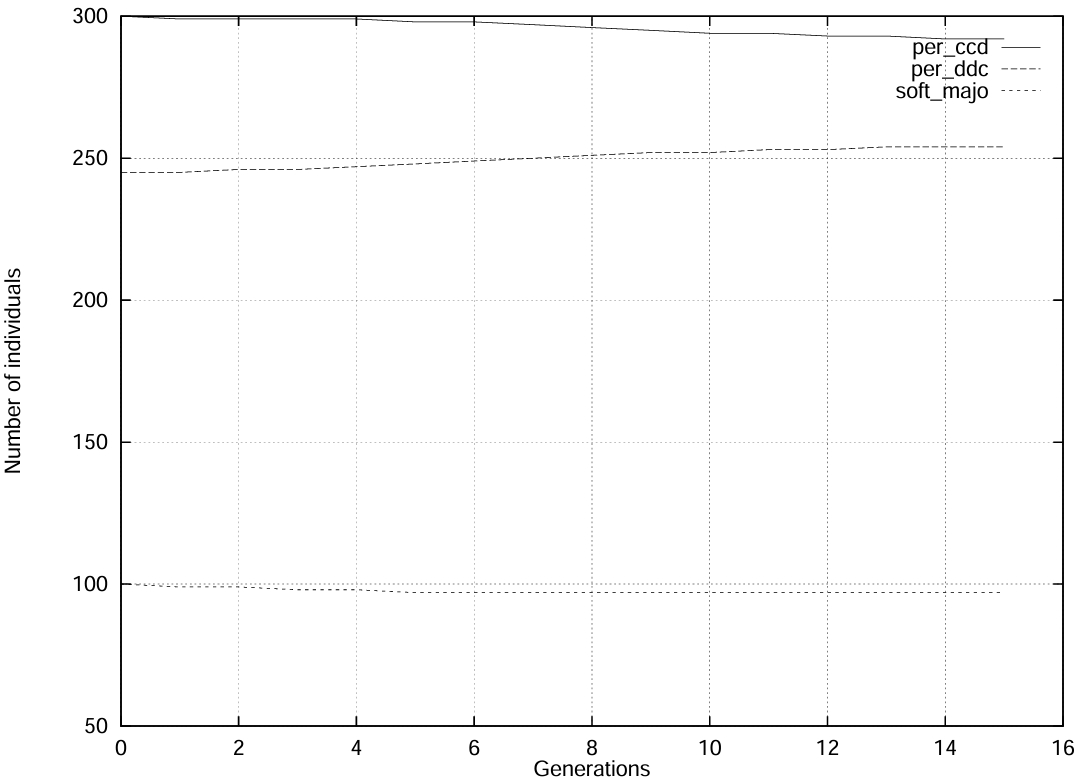
\includegraphics[width=0.7\textwidth]{RefPaperFigures/fig7b.jpeg}\par\vspace{0.5em}
	    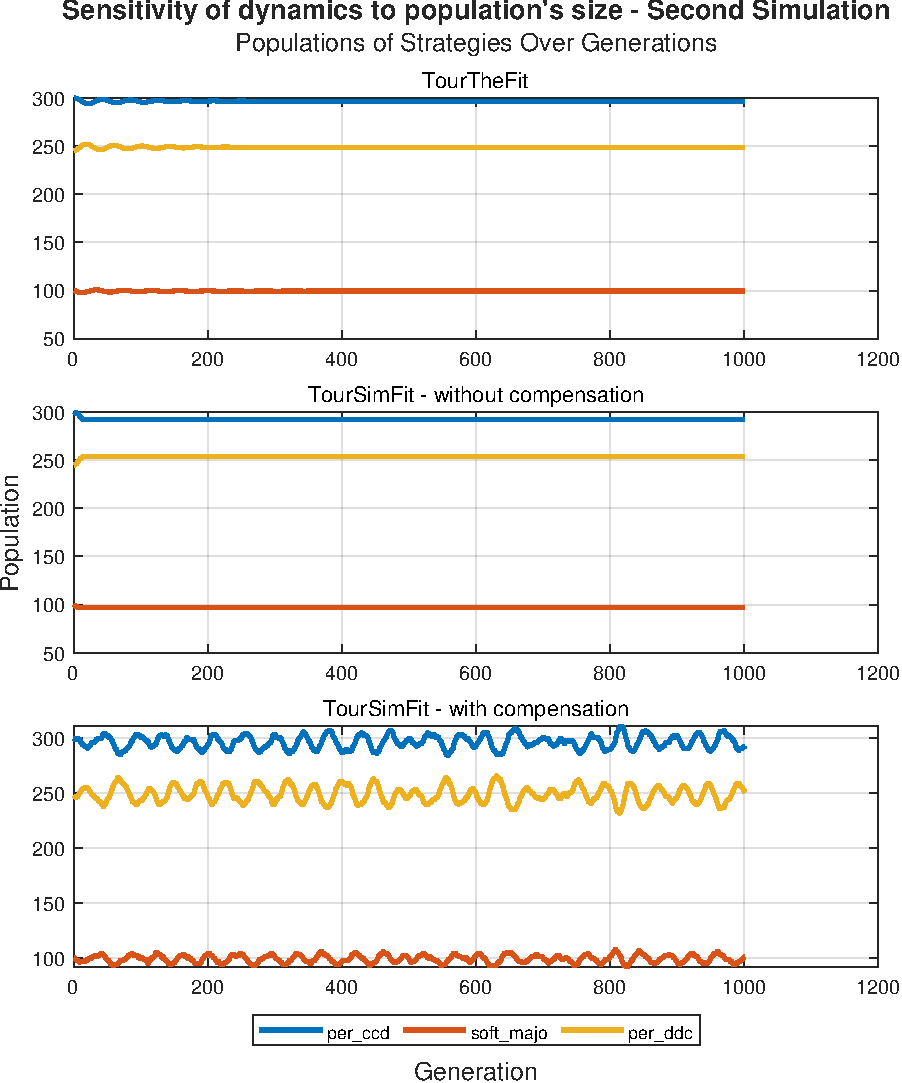
\includegraphics[width=0.7\textwidth]{Sensitivity of dynamics to population's size - Second Simulation.pdf}
	    \caption{8th Simulation - Sensitivity of dynamics to population's size - Second Simulation}
	    \label{fig:Sensitivity of dynamics to population's size - Second Simulation}
	\end{figure}
\subsubsection{9th Simulation - Sensitivity of winner to population's size - First Simulation}
	\begin{figure}[h]
	    \centering
		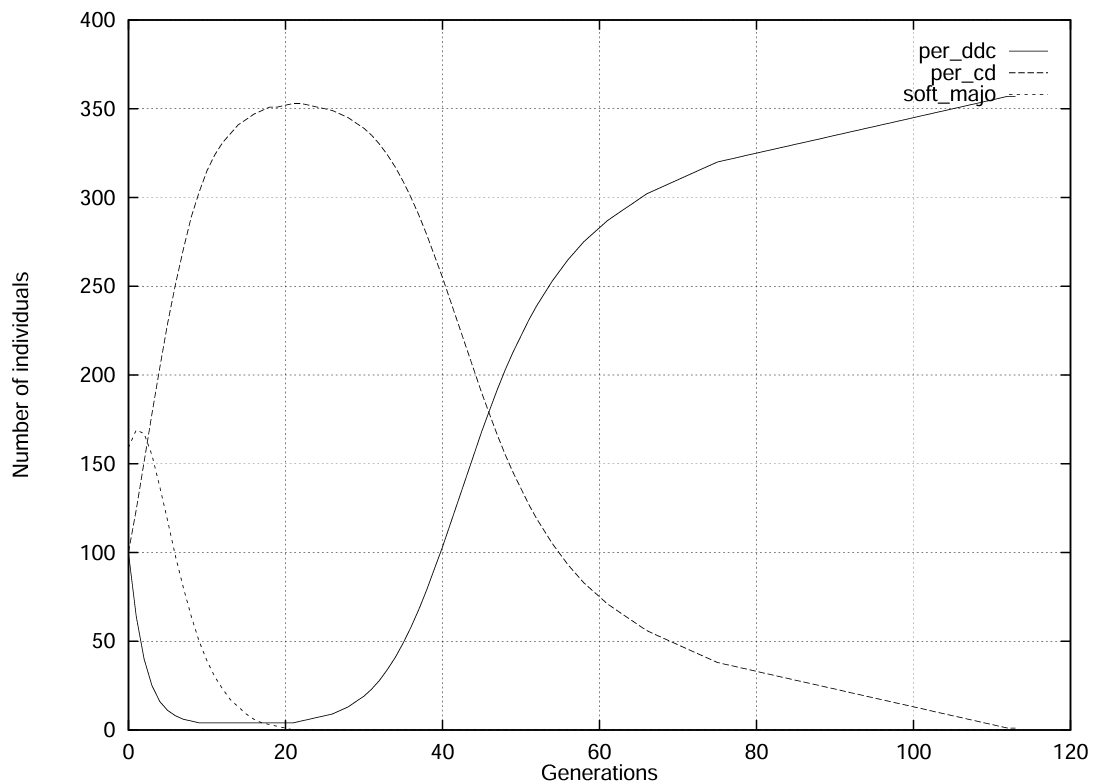
\includegraphics[width=0.7\textwidth]{RefPaperFigures/fig8a.jpeg}\par\vspace{0.5em}
	    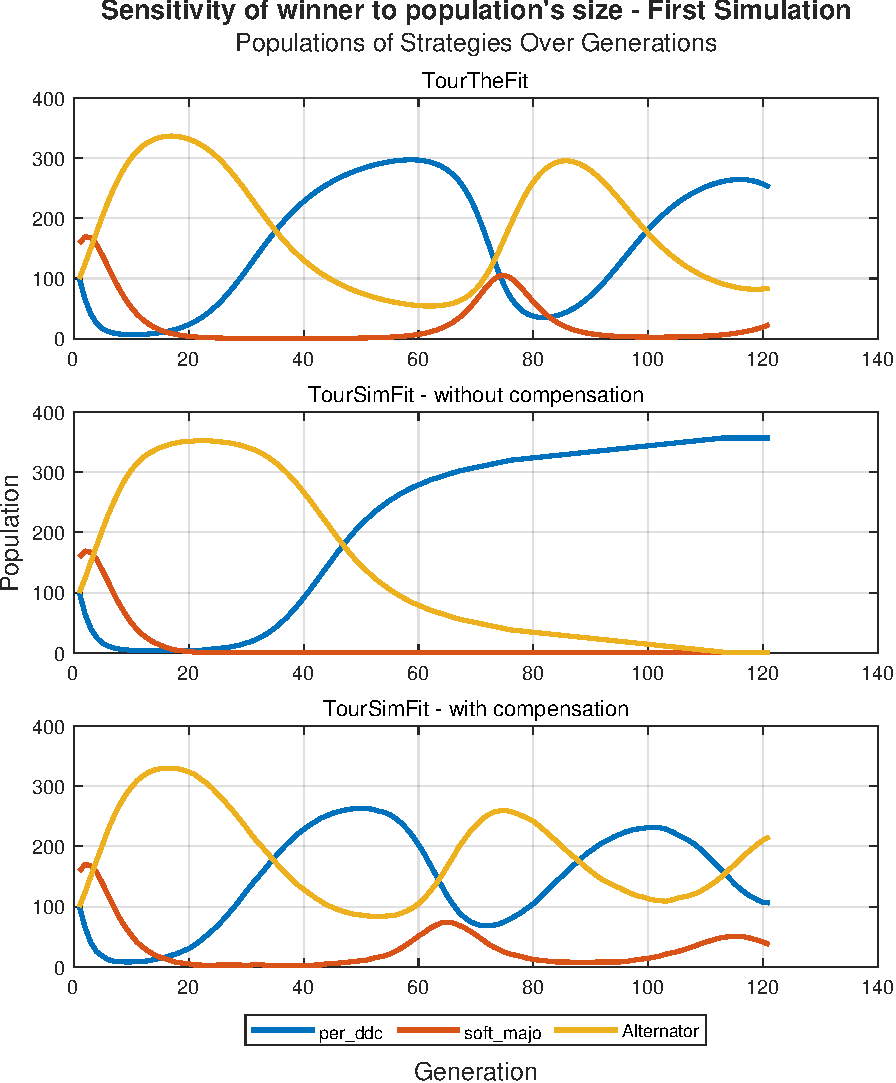
\includegraphics[width=0.7\textwidth]{Sensitivity of winner to population's size - First Simulation.pdf}
	    \caption{9th Simulation - Sensitivity of winner to population's size - First Simulation}
	    \label{fig:Sensitivity of winner to population's size - First Simulation}
	\end{figure}
\subsubsection{10th Simulation - Sensitivity of winner to population's size - Second Simulation}
	\begin{figure}[h]
	    \centering
		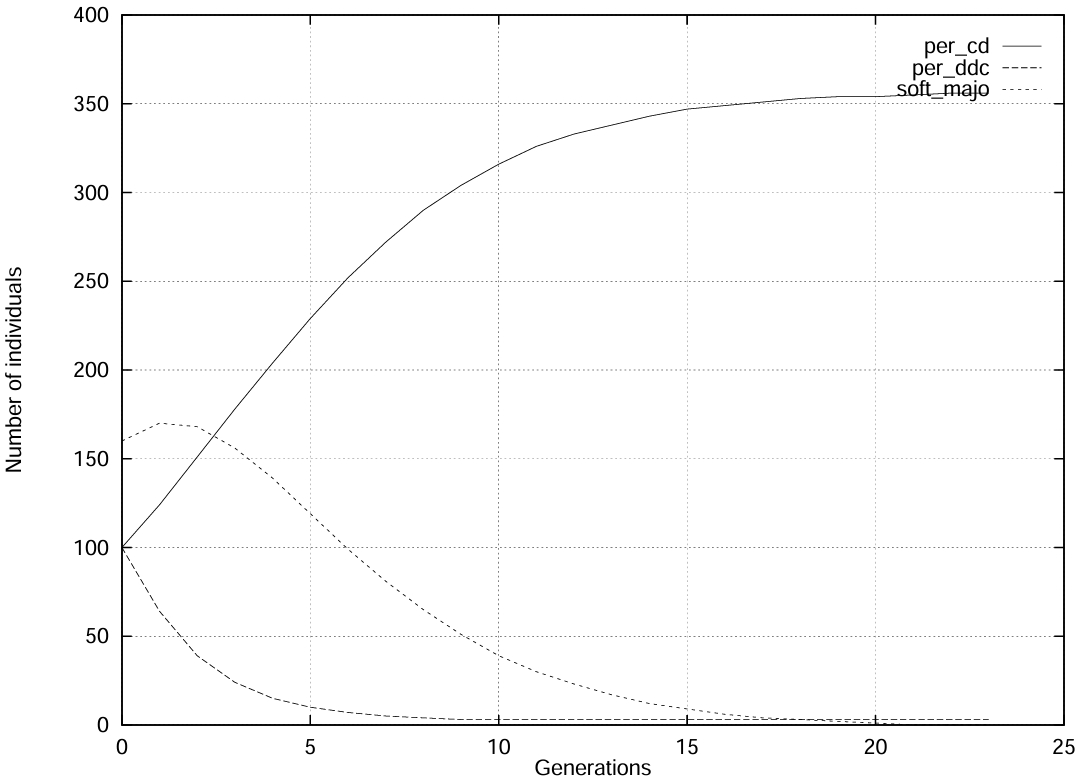
\includegraphics[width=0.7\textwidth]{RefPaperFigures/fig8b.jpeg}\par\vspace{0.5em}
	    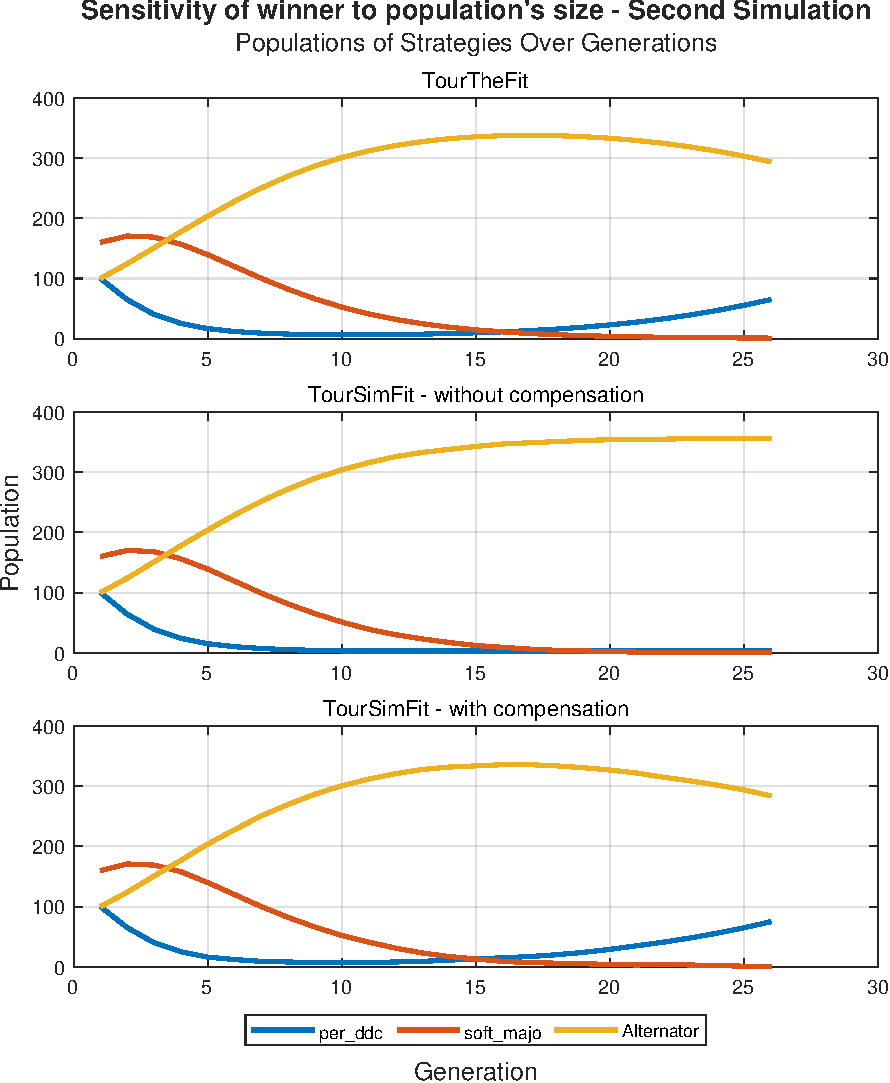
\includegraphics[width=0.7\textwidth]{Sensitivity of winner to population's size - Second Simulation.pdf}
	    \caption{10th Simulation - Sensitivity of winner to population's size - Second Simulation}
	    \label{fig:Sensitivity of winner to population's size - Second Simulation}
	\end{figure}
\subsubsection{11th Simulation - Sensitivity to game length - First Simulation}
	\begin{figure}[h]
	    \centering
		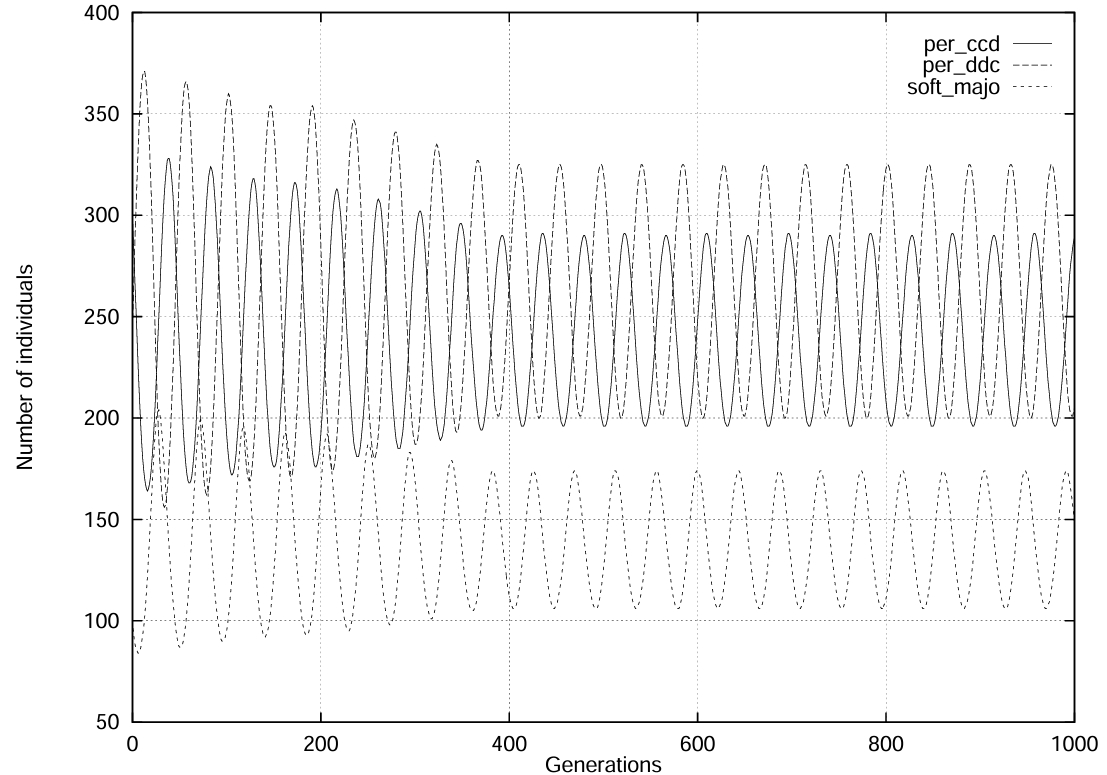
\includegraphics[width=0.7\textwidth]{RefPaperFigures/fig9a.jpeg}\par\vspace{0.5em}
	    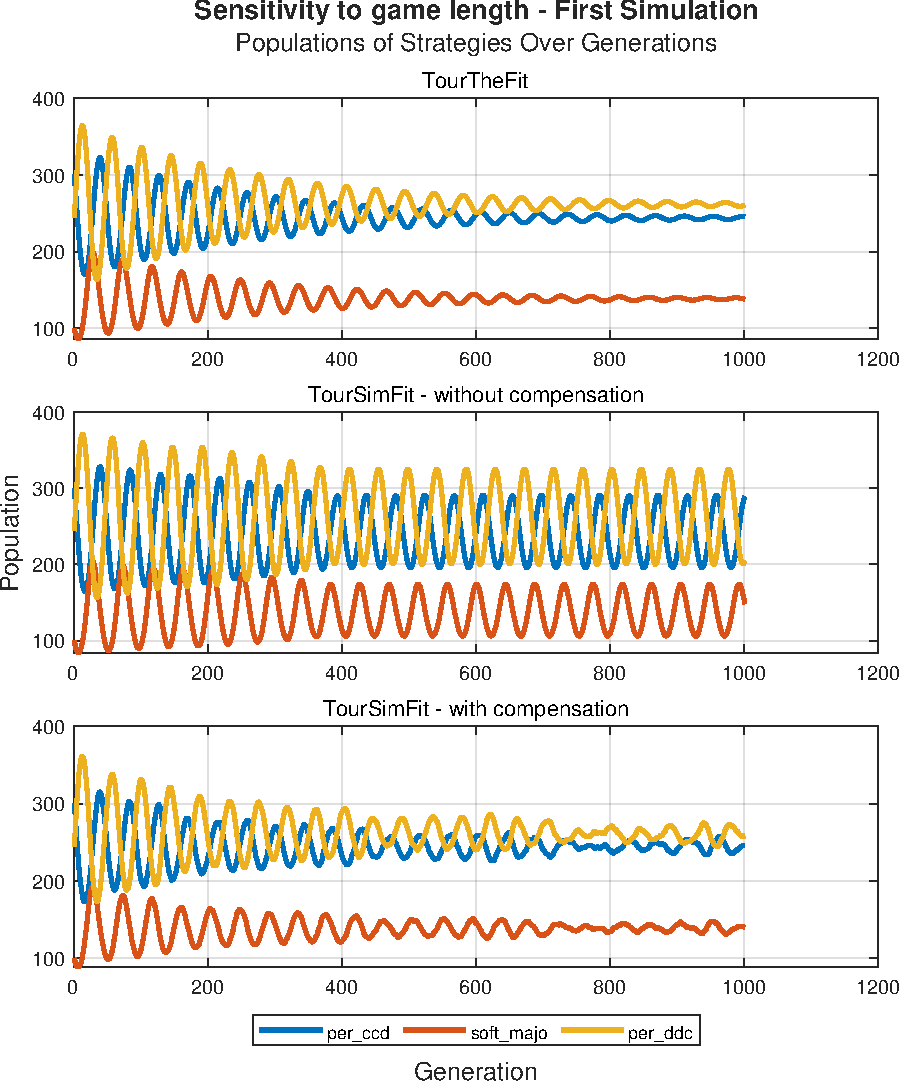
\includegraphics[width=0.7\textwidth]{Sensitivity to game length - First Simulation.pdf}
	    \caption{11th Simulation - Sensitivity to game length - First Simulation}
	    \label{fig:Sensitivity to game length - First Simulation}
	\end{figure}
\subsubsection{12th Simulation - Sensitivity to game length - Second Simulation}
	\begin{figure}[h]
	    \centering
		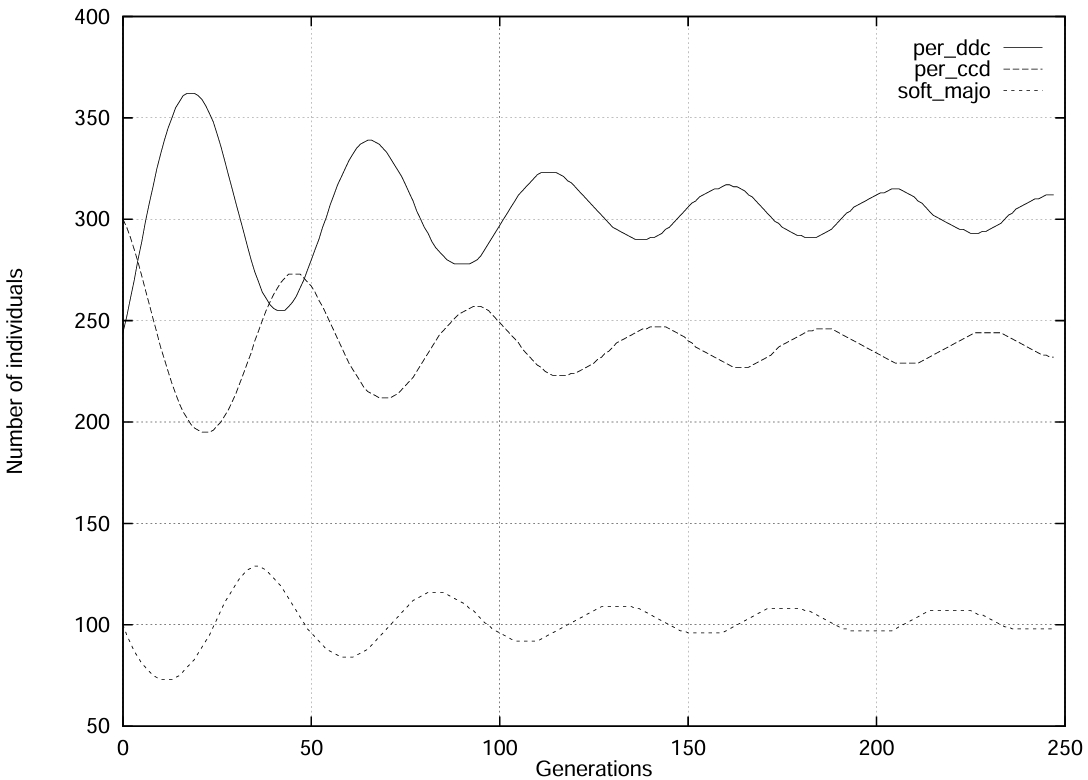
\includegraphics[width=0.7\textwidth]{RefPaperFigures/fig9b.jpeg}\par\vspace{0.5em}
	    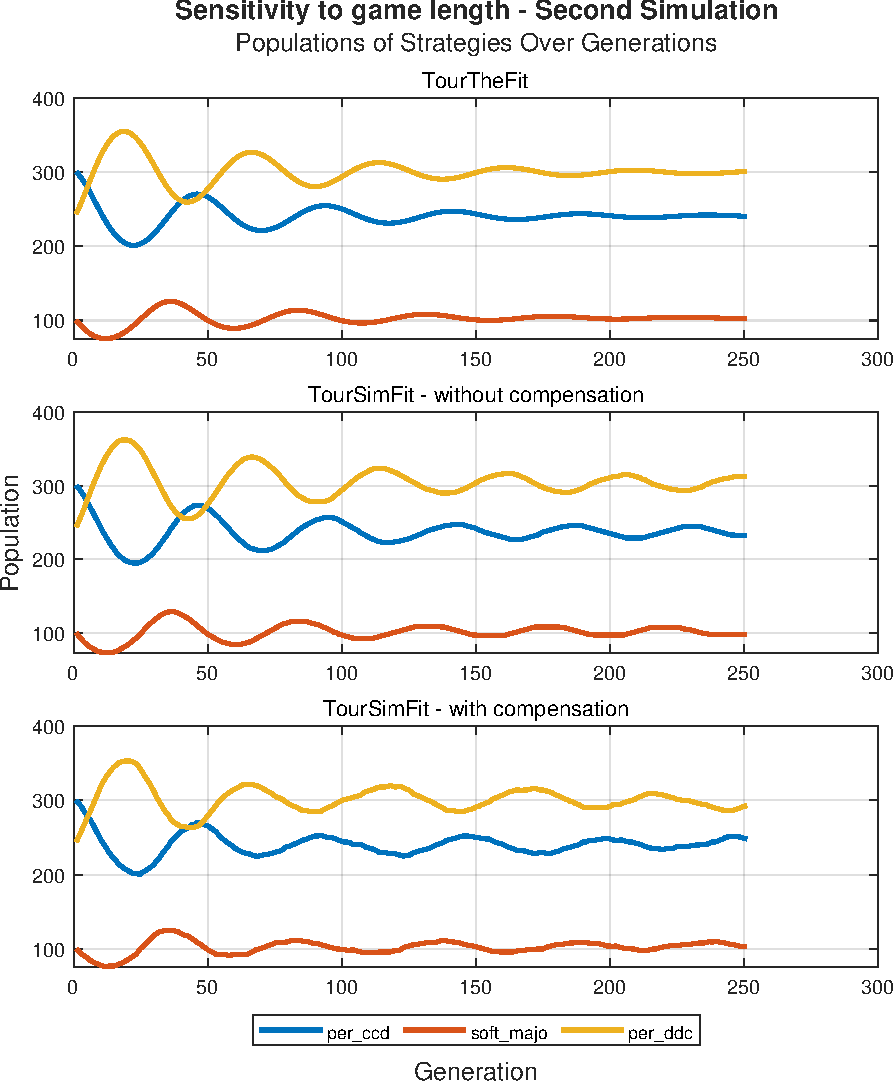
\includegraphics[width=0.7\textwidth]{Sensitivity to game length - Second Simulation.pdf}
	    \caption{12th Simulation - Sensitivity to game length - Second Simulation}
	    \label{fig:Sensitivity to game length - Second Simulation}
	\end{figure}
\subsubsection{13th Simulation - Sensitivity to CIPD payoff - First Simulation}
	\begin{figure}[h]
	    \centering
		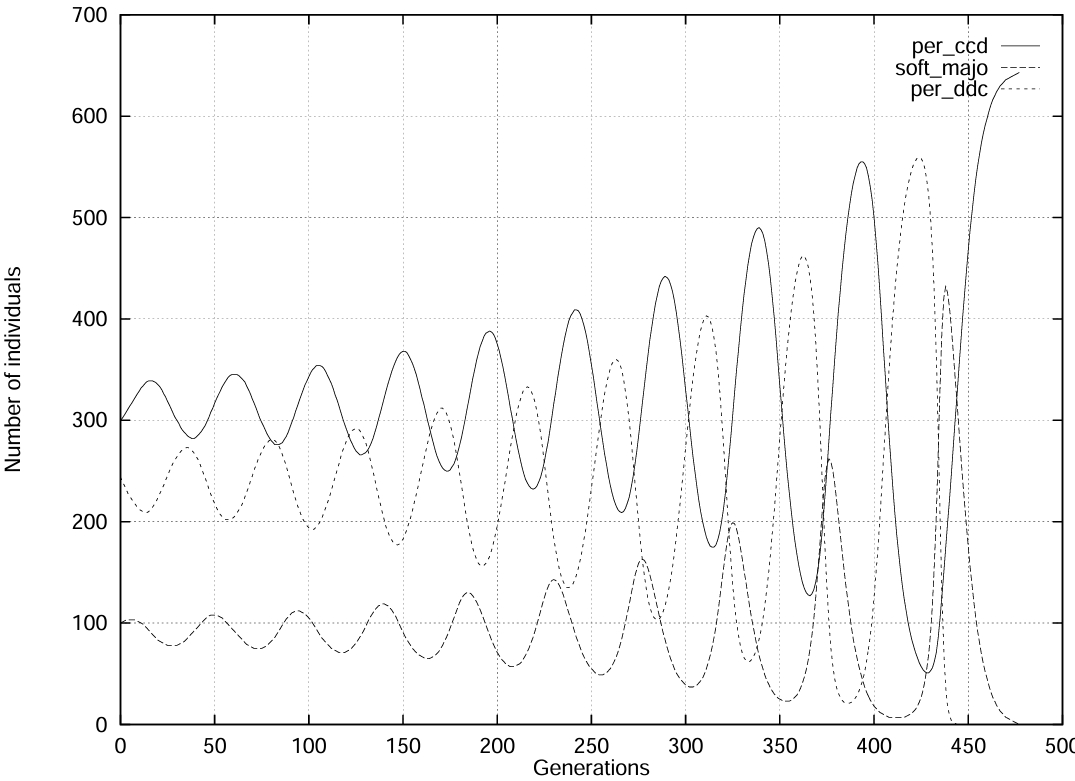
\includegraphics[width=0.7\textwidth]{RefPaperFigures/fig10a.jpeg}\par\vspace{0.5em}
	    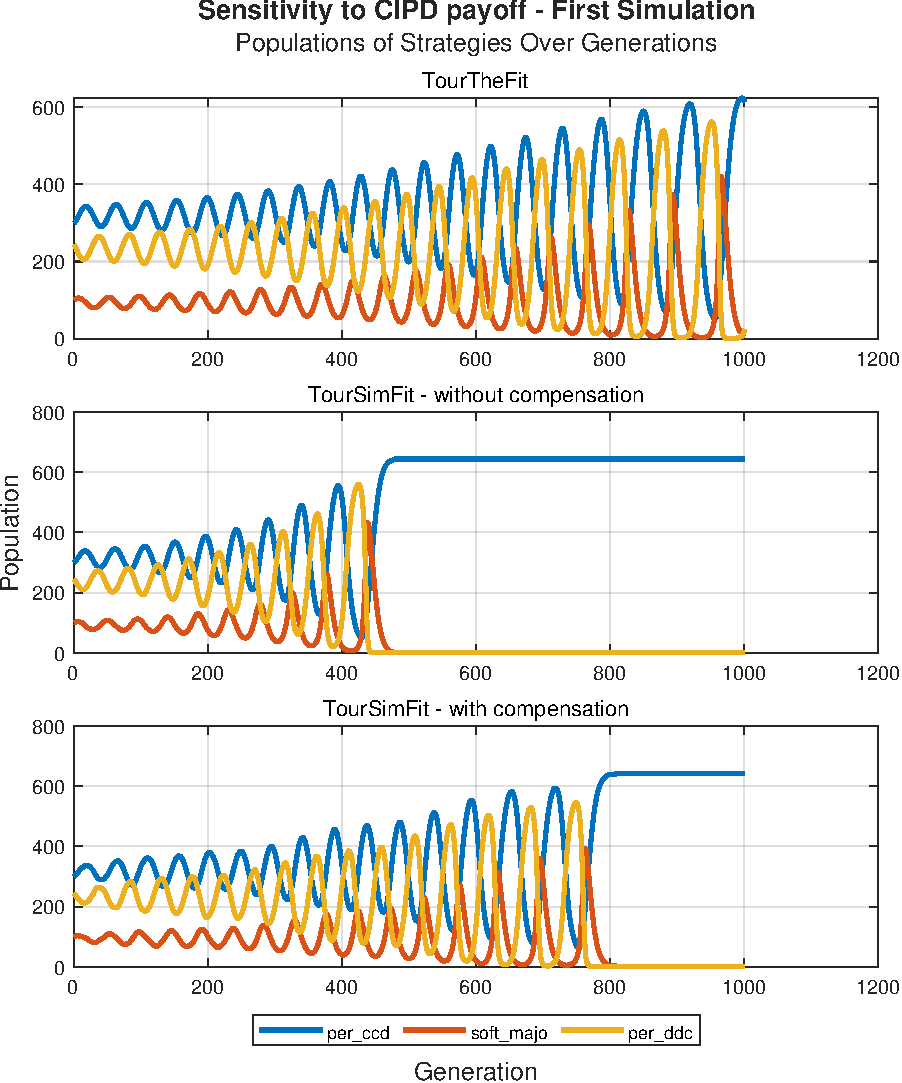
\includegraphics[width=0.7\textwidth]{Sensitivity to CIPD payoff - First Simulation.pdf}
	    \caption{13th Simulation - Sensitivity to CIPD payoff - First Simulation}
	    \label{fig:Sensitivity to CIPD payoff - First Simulation}
	\end{figure}
\subsubsection{14th Simulation - Sensitivity to CIPD payoff - Second Simulation}
	\begin{figure}[h]
	    \centering
		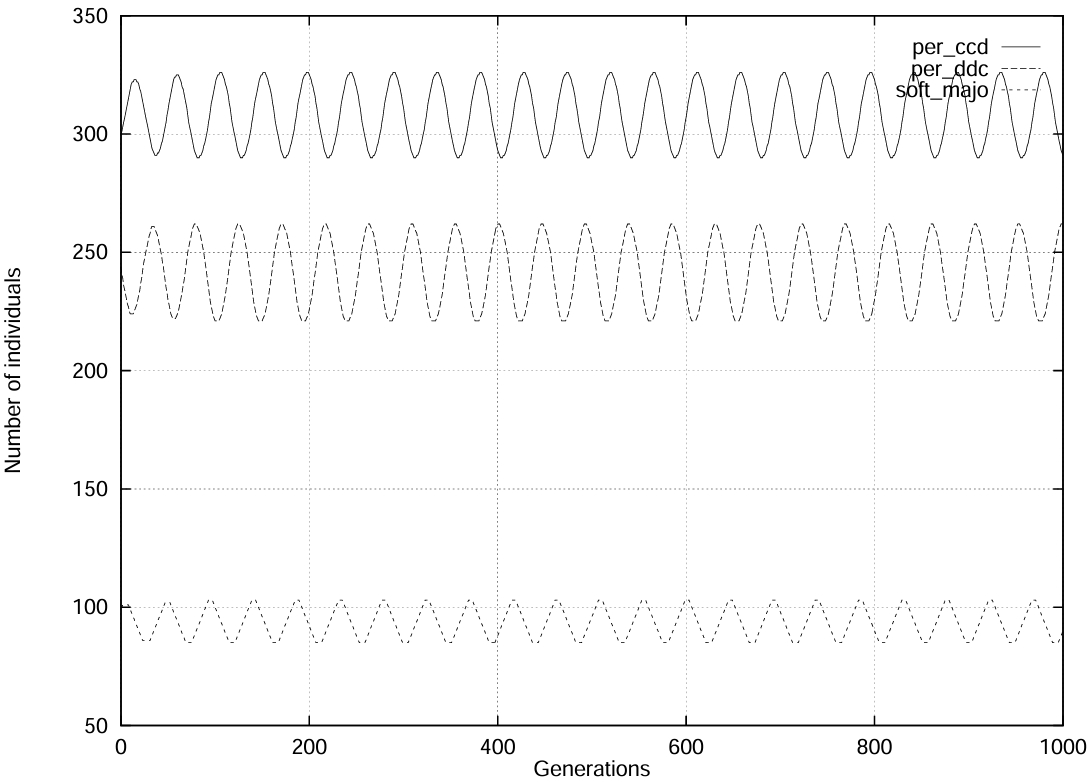
\includegraphics[width=0.7\textwidth]{RefPaperFigures/fig10b.jpeg}\par\vspace{0.5em}
	    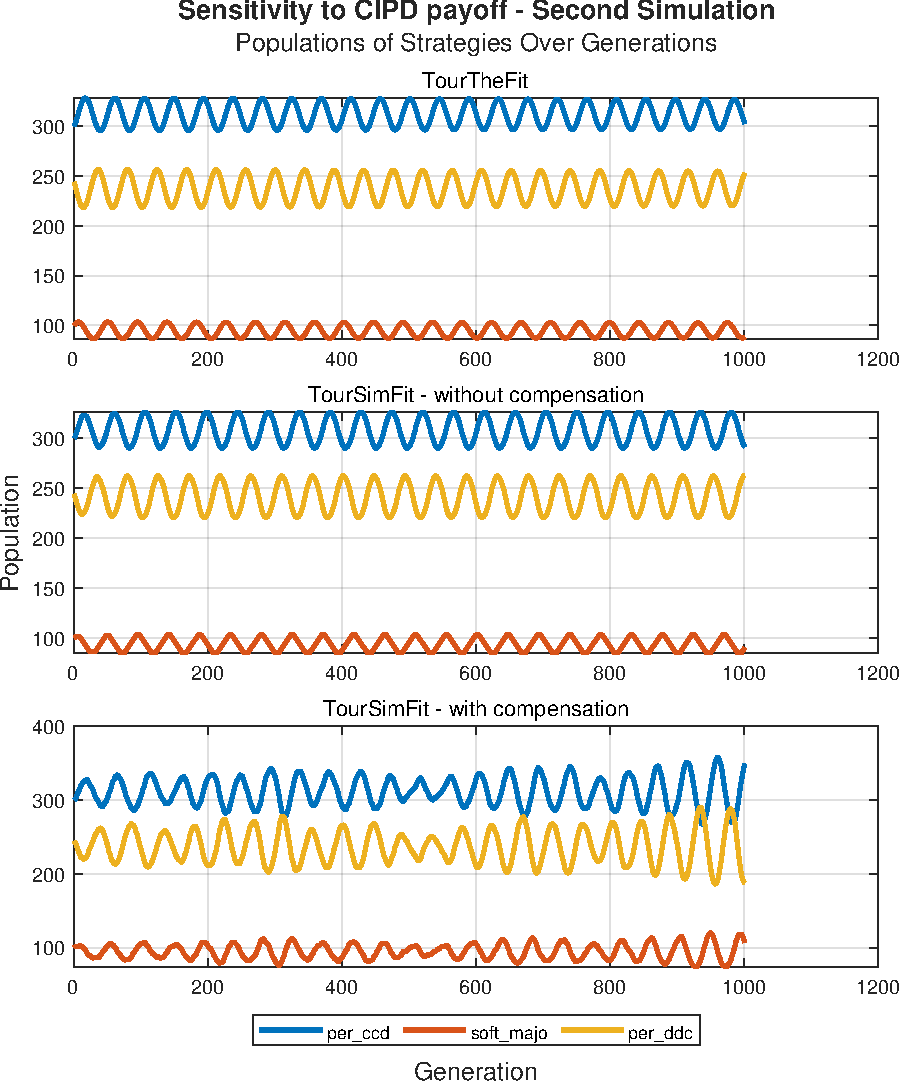
\includegraphics[width=0.7\textwidth]{Sensitivity to CIPD payoff - Second Simulation.pdf}
	    \caption{14th Simulation - Sensitivity to CIPD payoff - Second Simulation}
	    \label{fig:Sensitivity to CIPD payoff - Second Simulation}
	\end{figure}
\subsubsection{15th Simulation - Sensitivity to repartition computation method - First Simulation}
	\begin{figure}[h]
	    \centering
		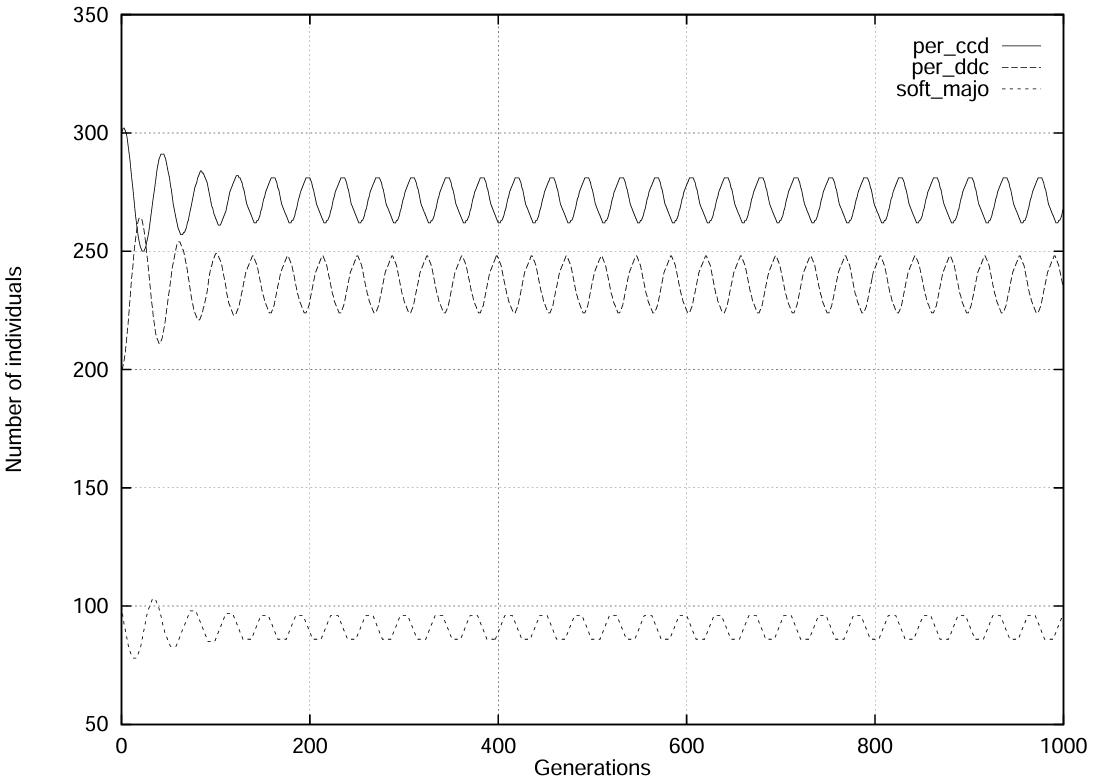
\includegraphics[width=0.49\textwidth]{RefPaperFigures/fig11a.jpeg}
		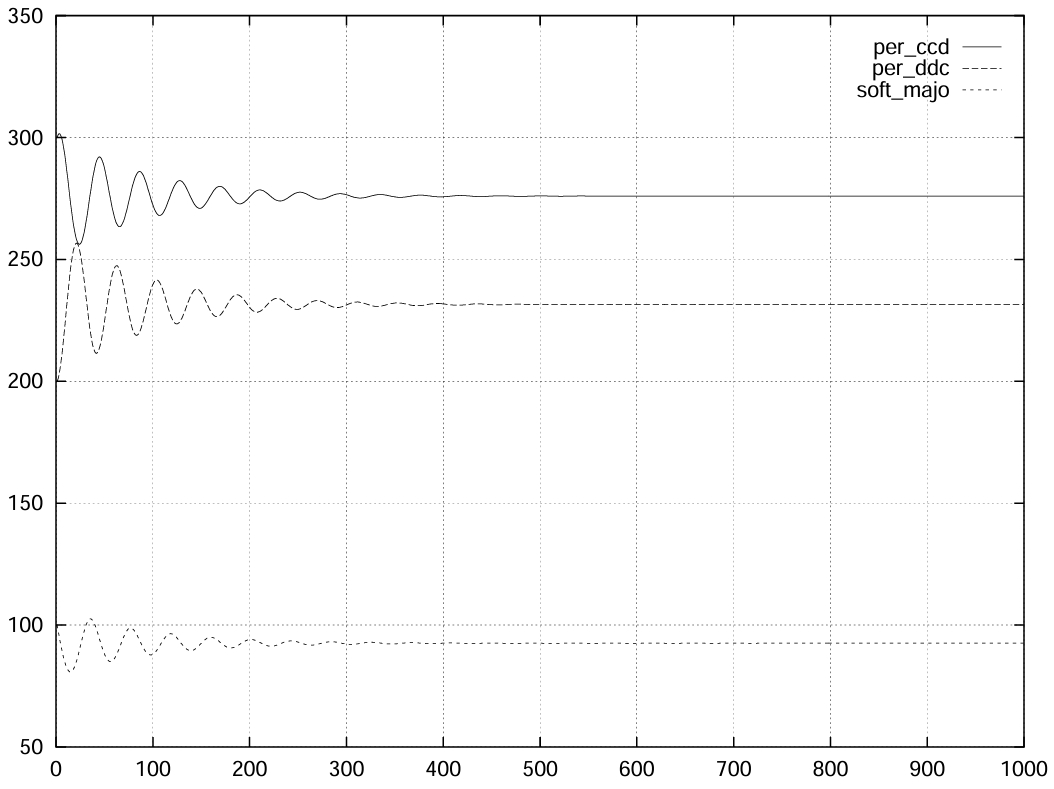
\includegraphics[width=0.49\textwidth]{RefPaperFigures/fig11b.jpeg}\par\vspace{0.5em}\par\vspace{0.5em}
	    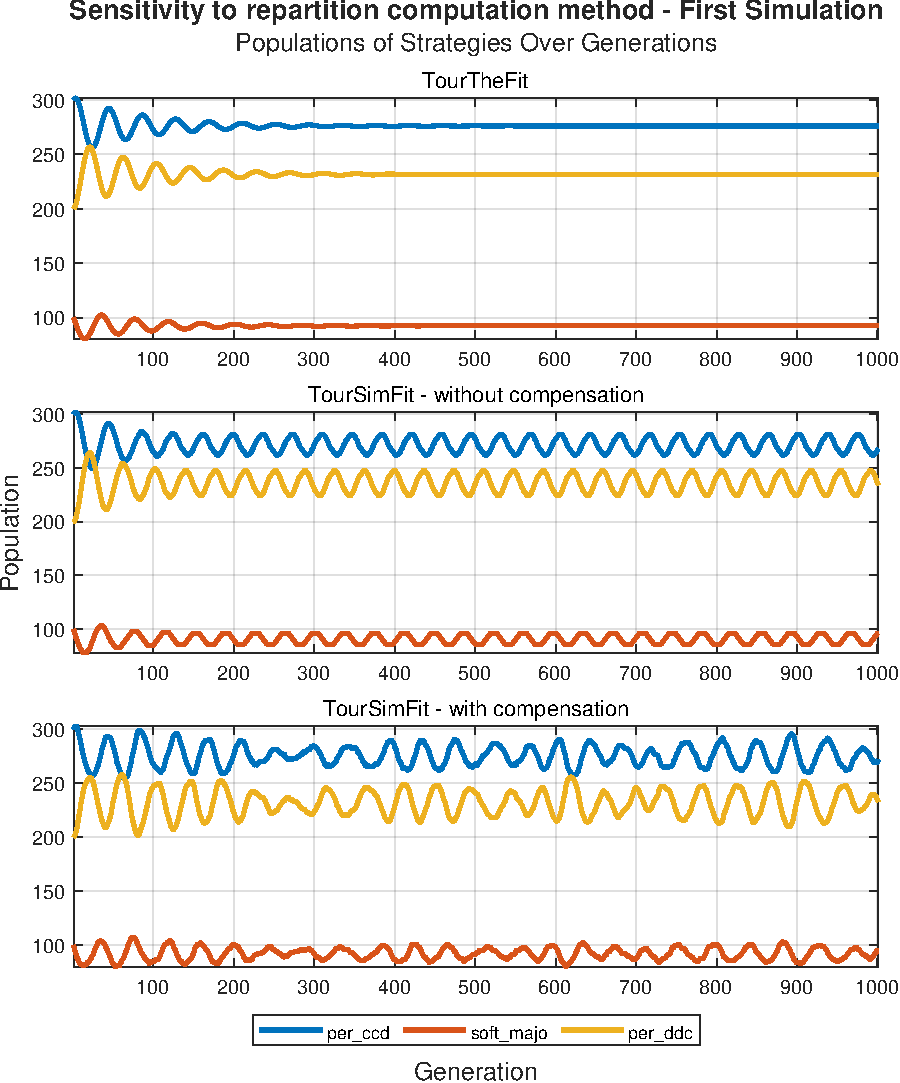
\includegraphics[width=0.7\textwidth]{Sensitivity to repartition computation method - First Simulation.pdf}
	    \caption{15th Simulation - Sensitivity to repartition computation method - First Simulation}
	    \label{fig:Sensitivity to repartition computation method - First Simulation}
	\end{figure}
\subsubsection{16th Simulation - Sensitivity to repartition computation method - Second Simulation}
	\begin{figure}[h]
	    \centering
		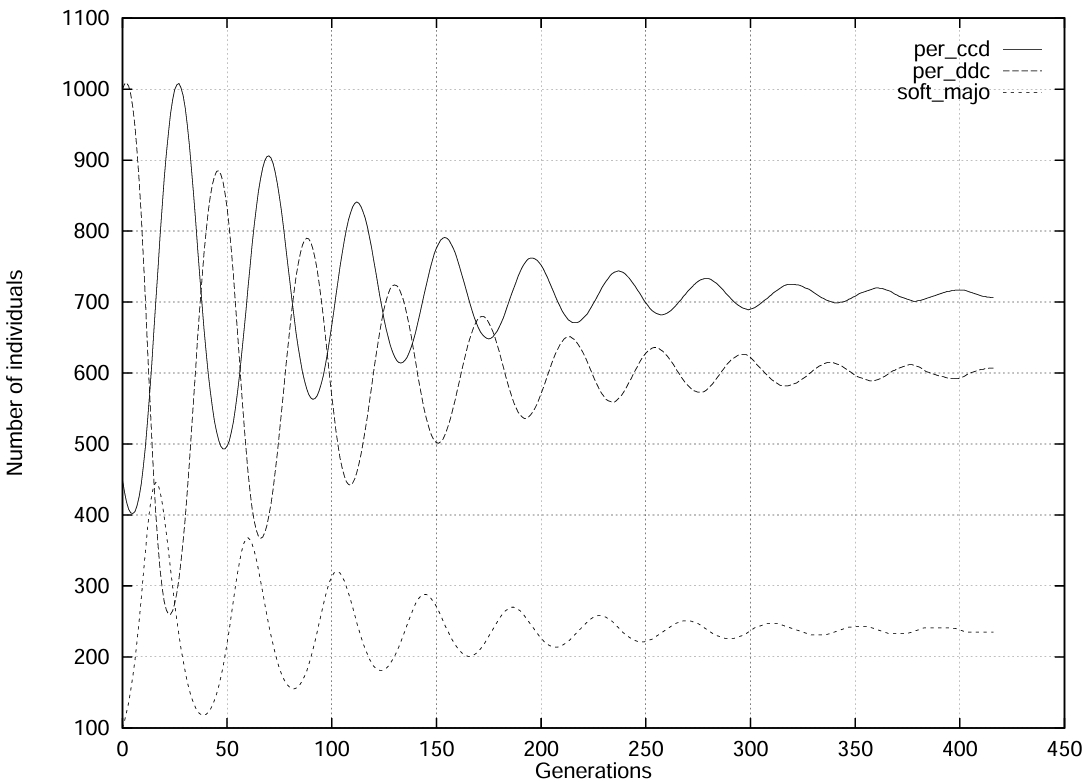
\includegraphics[width=0.7\textwidth]{RefPaperFigures/fig12a.jpeg}\par\vspace{0.5em}
	    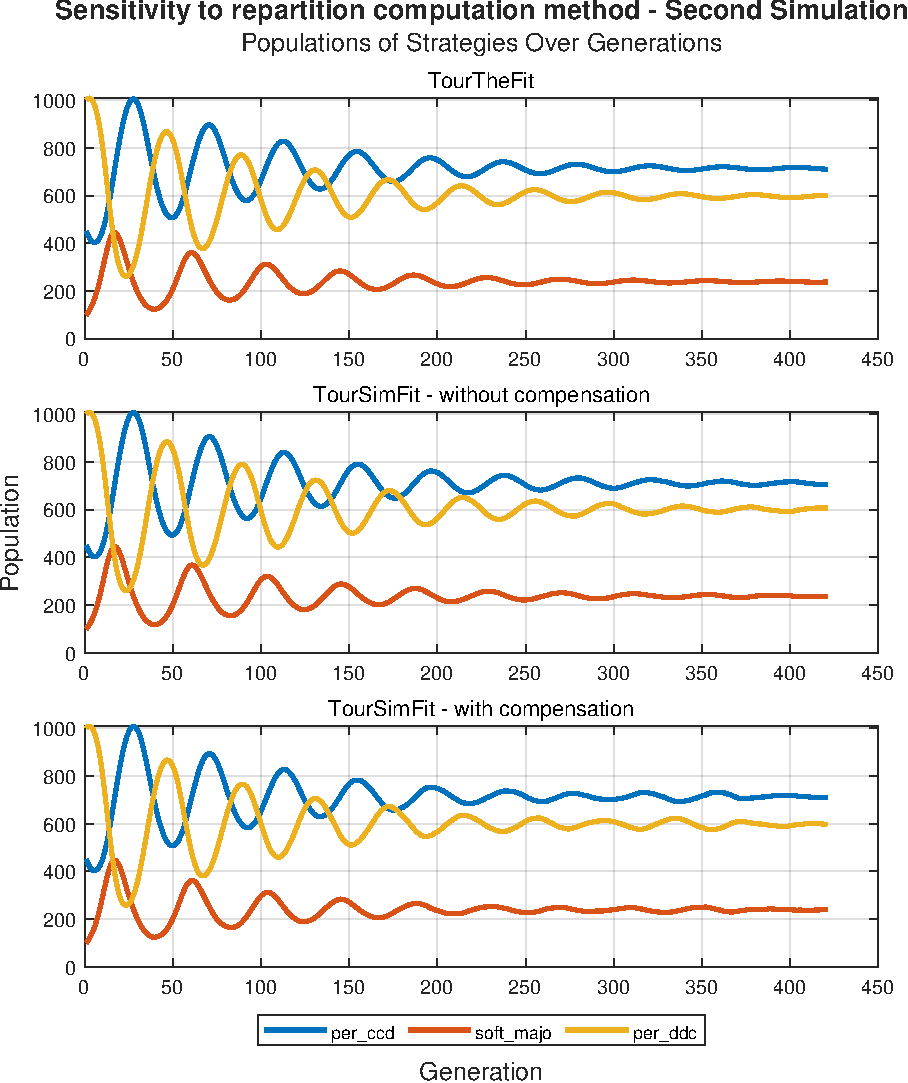
\includegraphics[width=0.7\textwidth]{Sensitivity to repartition computation method - Second Simulation.pdf}
	    \caption{16th Simulation - Sensitivity to repartition computation method - Second Simulation}
	    \label{fig:Sensitivity to repartition computation method - Second Simulation}
	\end{figure}
\subsubsection{17th Simulation - Sensitivity to repartition computation method - Third Simulation}
	\begin{figure}[h]
	    \centering
		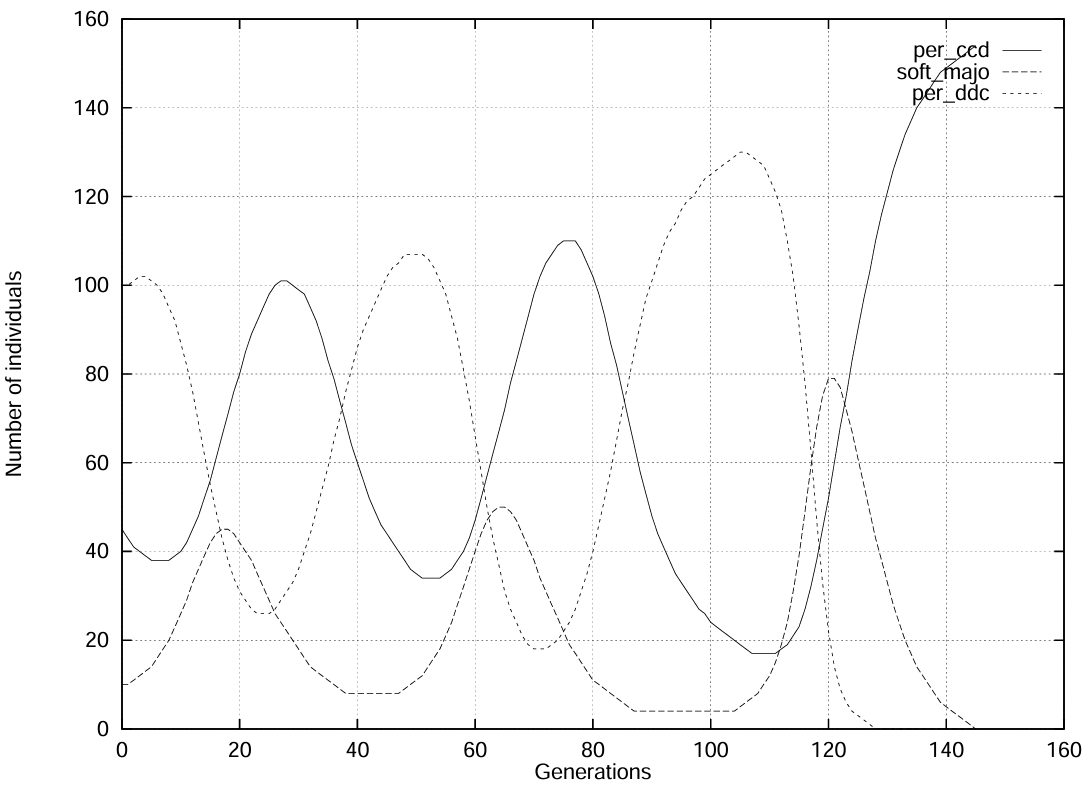
\includegraphics[width=0.7\textwidth]{RefPaperFigures/fig12b.jpeg}\par\vspace{0.5em}
	    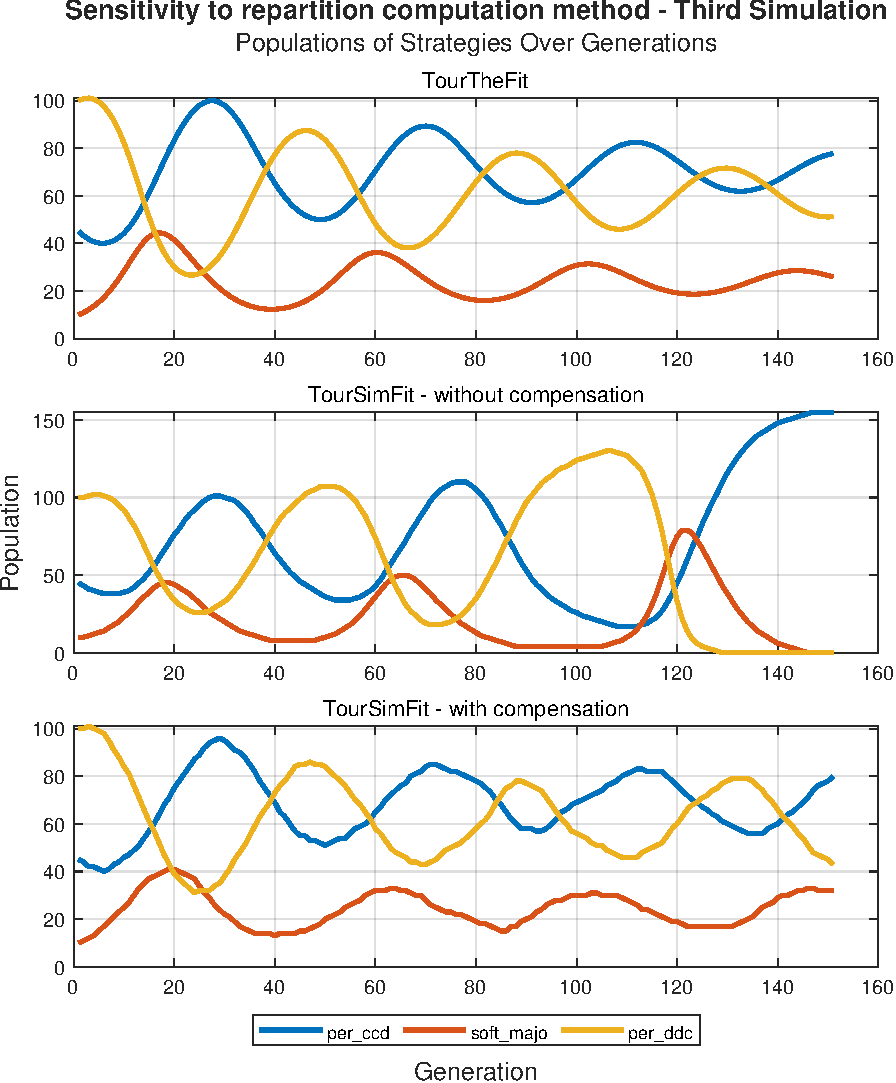
\includegraphics[width=0.7\textwidth]{Sensitivity to repartition computation method - Third Simulation.pdf}
	    \caption{17th Simulation - Sensitivity to repartition computation method - Third Simulation}
	    \label{fig:Sensitivity to repartition computation method - Third Simulation}
	\end{figure}
\clearpage
\section{Imitation Dynamics}
Η δεύτερη εξελικτική δυναμική που θα παρουσιαστεί είναι αυτή των Imitation Dynamics - δυναμική μίμησης. Στην περίπτωση αυτή, δεν υπολογίζεται η νέα κατανομή του πληθυσμού αυστηρά ως συνάρτηση του fitness της κάθε στρατηγικής για κάθε γενιά, αλλά υιοθετείται μία πιο απλή και ίσως πιο εφαρμόσιμη στην πραγματικότητα λογική: σε κάθε γενιά, βρίσκουμε τη στρατηγική (ή σε περίπτωση ισοπαλίας τις στρατηγικές) που ανταποκρίθηκαν καλύτερα. Έπειτα, έχοντας ορίσει τον αριθμό K των παικτών που αλλάζουν στρατηγική ανά γενιά, επιλέγονται τυχαία K παίκτες μη βέλτιστης στρατηγικής και υιοθετούν μία εκ των βέλτιστων στρατηγικών, πάλι τυχαία, σε περίπτωση ισοβαθμίας. 

Να επισημανθεί ότι η επιλογή γίνεται μόνο μεταξύ παικτών μη βέλτιστης στρατηγικής και όχι μεταξύ όλων των παικτών του πληθυσμού. Αυτό θεωρούμε πως ανταποκρίνεται περισσότερο στην πραγματικότητα - αν βρίσκεται κάποιος παίκτης ήδη στη βέλτιστη στρατηγική, γιατί να σκεφτεί να αλλάξει στρατηγική; Η επιλογή αυτή έχει μερικές συνέπειες στα αποτελέσματα που παρουσιάζονται παρακάτω.

Για την εύρεση της βέλτιστης στρατηγικής χρησιμοποιείται υπολογισμός του score παρόμοιος με αυτόν της περίπτωσης των fitness dynamics, ώστε να εξοικονομείται χρόνος κατά την εκτέλεση τως προγραμμάτων. Δηλαδή, δεν προσομοιώνονται πραγματικά τα matches μεταξύ κάθε παίκτη, αλλά υπολογίζονται τα scores με βάση τις απολαβές κάθε στρατηγικής εναντίον κάθε στρατηγικής και τους αντίστοιχους πληθυσμούς.

Όπως θα παρουσιαστεί παρακάτω, κατά τη θεωρητική παρουσίαση της συνάρτησης TourTheImi, η διαδικασία αυτή μπορεί να διατυπωθεί με τη βοήθεια μαρκοβιανής αλυσίδας, όπου καταστάσεις είναι οι διάφορες πιθανές κατανομές πληθυσμού, με βάση το άθροισμα των αρχικών πληθυσμών (τον συνολικό πληθυσμό) και τον αριθμό στρατηγικών που εμπλέκονται στη διαδικασία. Στην αναφορά του κ. Κεχαγιά βρίσκεται το θεωρητικό υπόβαθρο αυτών που θα συζητηθούν αργότερα: θεωρούμε αρχικά την r-state μαρκοβιανή αλυσίδα, όπου κάθε κατάσταση είναι η στρατηγική του κάθε παίκτη ξεχωριστά, π.χ. για N = 5 παίκτες και 3 στρατηγικές, πιθανό r-state είναι το (11323). Θεωρούμε έπειτα, τις s-states, όπου κατάσταση είναι ο πληθυσμός της κάθε στρατηγικής, στο προηγούμενο παράδειγμα το s-state θα ήταν (212). Ουσιαστικά πρόκειται για grouping διάφορων r-states σε ένα s-state, το οποίο, λόγω του ότι δε μας ενδιαφέρει πραγματικά ο κάθε παίκτης ξεχωριστά, αλλά ο συνολικός πληθυσμός της κάθε στρατηγικής, είναι ισοδύναμο. Αποδεικνύεται ότι η διαδικασία r(t) είναι lumpable και άρα ότι η s(t) είναι μαρκοβιανή αλυσίδα. Η θεωρητική αυτή γνώση είναι απαραίτητη για την υλοποίηση της TourTheImi παρακάτω.
\subsection{Η συνάρτηση TourSimImi}
Υλοποιείται, αρχικά, συνάρτηση προσομοίωσης του εξελικτικού πρωταθλήματος με δυναμική μίμησης [POP, BST]\- =\- TourSimImi\- (B,\- Strategies,\- POP0,\- K,\- T, \-J, \- mode). Οι είσοδοι και έξοδοι της συνάρτησης είναι όμοιες με αυτές της TourSimFit, με έξτρα όρισμα μία ακέραια τιμή K που προσδιορίζει τον αριθμό παικτών που αλλάζουν στρατηγική ανά γενιά. Το έξτρα όρισμα mode (η συνάρτηση τρέχει με default τιμή "Individual") λαμβάνει τιμές "Individual" και "Total" και αναφέρεται στον τρόπο με τον οποίο επιλέγεται η βέλτιστη στρατηγική: στην περίπτωση "Individual", επιστρέφεται απλά η στρατηγική του καλύτερου παίκτη, ενώ στην περίπτωση "Total" επιστρέφεται η στρατηγική με το μεγαλύτερο άθροισμα scores ανά τους παίκτες που τη χρησιμοποιούν. Η επιλογή του mode επιφέρει σημαντικά διαφορετικά αποτελέσματα, όπως θα παρουσιαστεί παρακάτω.

Να σχολιαστεί επίσης ότι, σε περίπτωση που οι παίκτες με μη βέλτιστη στρατηγική είναι λιγότεροι από K, αλλάζουν στρατηγική όλοι οι παίκτες με μη βέλτιστη στρατηγική, σε πλήθος λιγότεροι από K. Παραδείγματος χάριν, βρισκόμαστε σε κατάσταση μόνο με All\_C και TitForTat, οι απολαβές με τη μέθοδο Individual είναι ίδιες και το $K = 1$. Υπάρχουν 0 άτομα με μη βέλτιστη στρατηγική, άρα δεν αλλάζει κανένας στρατηγική, μιας και $0<1$. Αντίστοιχα, αν οι μη βέλτιστοι παίκτες είναι 2 και το K είναι 3, θα αλλάξουν μόνο οι 2 και ούτω καθεξής.

\subsection{Η συνάρτηση TourTheImi}
Η συνάρτηση TourTheImi είναι το τελευταίο ζητούμενο της εργασίας. Έχει τη μορφή P\- =\- TourTheImi\- (B,\- Strategies,\- POP0,\- K,\- T,\- J,\- mode), με ορίσματα πλήρως πανομοιότυπα της συνάρτησης TourSimImi και έξοδο τον πίνακα μεταβάσεων της μαρκοβιανής αλυσίδας των s-states P. Στην πραγματικότητα, για τον υπολογισμό του πίνακα P, ο αρχικός πληθυσμός χρησιμοποιείται μόνο για να υπολογιστεί ο συνολικός πληθυσμός του πρωταθλήματος (άρα θα μπορούσε απλά να αντικατασταθεί από ένα όρισμα N) και ο αριθμός γενεών J δε χρησιμοποιείται καθόλου.

Για την ανάλυση αυτή θεωρούμε τα s-states του πρωταθλήματος ως τους αριθμούς των παικτών κάθε στρατηγικής, π.χ. για N = 9 έχουμε $s_1 = \begin{bmatrix} 0 & 0 & 9 \end{bmatrix}$, $s_2 = \begin{bmatrix} 0 & 1 & 8 \end{bmatrix}$ και ούτω καθεξής. Ανάλογα με το όρισμα mode, αναμένουμε ο πίνακας μετάβασης να έχει διαφορετική μορφή. Για παράδειγμα, στο mode Individual και με στρατηγικές All\_D, All\_C, και TitForTat, η κατάσταση $\begin{bmatrix} 0 & 5 & 4 \end{bmatrix}$ αναμένουμε να είναι absorbing, μιας και δεν υπάρχουν μη βέλτιστοι παίκτες και άρα να έχει μόνο μία μετάβαση, στον εαυτό της, με πιθανότητα 1. Αντίθετα, στην περίπτωση Total, η κατάσταση αυτή δε θα ήταν absorbing, καθώς η στρατηγική All\_C συγκεντρώνει περισσότερους συνολικούς πόντους.

Δημιουργείται και μία ακόμη συνάρτηση AnalyzeMarkovChain\- (P,\- POP0,\- Str\-at\-e\-gies,\- Title), η οποία είναι υπεύθυνη για την παραγωγή των διαγραμμάτων μετάβασης καταστάσεων που παρουσιάζονται παρακάτω. Η συνάρτηση αυτή, με βάση τον πίνακα P που υπολογίζεται από τη συνάρτηση TourTheImi και τον αρχικό πληθυσμό POP0, διαχωρίζει τις καταστάσεις σε μεταβατικές - transient, απορροφητικές - absorbing και την αρχική κατάσταση. Επίσης, κάνει την περαιτέρω διάκριση μεταξύ reachable και unreachable καταστάσεων με βάση την αρχική κατάσταση. Δημιουργεί διάγραμμα της κάθε κατάστασης, στο οποίο φαίνεται με χρώμα ο τύπος κατάστασης, φαίνονται οι πληθυσμοί της κάθε κατάστασης, τα ονόματα των στρατηγικών, που δίνονται με το όρισμα Strategies, και οι αντίστοιχες πιθανότητες μετάβασης πάνω από κάθε μετάβαση. Το όρισμα Title είναι ο τίτλος του διαγράμματος που προκύπτει. 
\subsection{Προσομοιώσεις}
Παρακάτω παρουσιάζονται κάποιες προσομοιώσεις οι οποίες παράγονται από τις συναρτήσεις που περιγράφηκαν παραπάνω και παρουσιάζουν ενδιαφέρον. Η κάθε προσομοίωση βρίσκεται στο αρχείο example.m σε κατάλληλο Section και με Run Section προκύπτουν ακριβώς τα αποτελέσματα που παρουσιάζονται παρακάτω.
\subsubsection{1η Προσομοίωση - Παράδειγμα χρήσης των Tour\-The\-Imi, Analyze\-Markov\-Chain και Tour\-Sim\-Imi}
Στην πρώτη προσομοίωση \ref{fig:TourTheImi153} παρουσιάζεται η μαρκοβιανή αλυσίδα που προκύπτει για τις στρατηγικές $\begin{bmatrix}All\_D&All\_C&TitForTat\end{bmatrix}$ σε μείγμα $\begin{bmatrix}1&5&3\end{bmatrix}$.
Από το διάγραμμα που προκύπτει παρατηρούμε ότι οι πιθανές απορροφητικές καταστάσεις είναι η $\begin{bmatrix}9&0&0\end{bmatrix}$, δηλαδή η επικράτηση της στρατηγικής $All\_D$, η $\begin{bmatrix}0&0&9\end{bmatrix}$, δηλαδή η επικράτηση της στρατηγικής $TitForTat$ και η $\begin{bmatrix}0&1&8\end{bmatrix}$, δηλαδή η επικράτηση της $TitForTat$ αλλά με επιβίωση της $All\_C$. Από τις πιθανότητες μετάβασης, που απεικονίζονται στα βέλη των μεταβάσεων, παρατηρούμε ότι η τελευταία απορροφητική κατάσταση έχει σημαντικά χαμηλότερη πιθανότητα να συμβεί σε σχέση με τις άλλες δύο. Ακόμη παρατηρούμε ότι οι καταστάσεις στις οποίες υπάρχουν μόνο οι συμπαθείς στρατηγικές ($All\_C$ και $TitForTat$), δηλαδή στρατηγικές οι οποίες ποτέ δεν λιποτακτούν πρώτες και άρα οι παίκτες των οποίων αποκτούν ίσα σκορ παίζοντας μεταξύ τους, μεταβαίνουν μόνο στον εαυτό τους καθώς δεν υπάρχουν παίκτες με σκορ χαμηλότερο του μεγίστου.

	\begin{figure}[h]
	      \centering
	      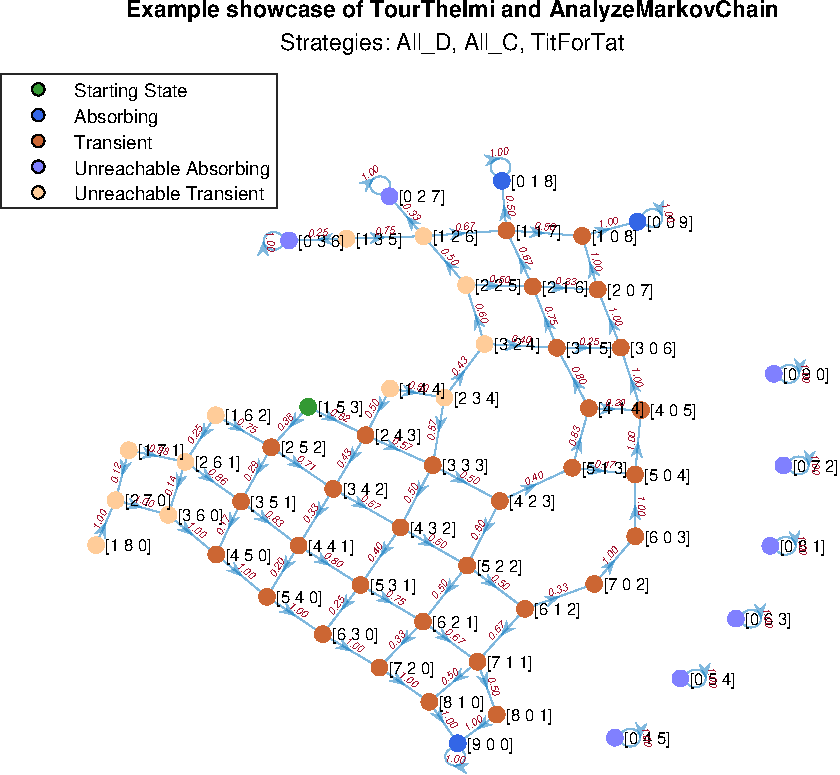
\includegraphics[width=0.95\textwidth]{Example showcase of TourTheImi and AnalyzeMarkovChain.pdf}
	      \caption{Example showcase of TourTheImi and AnalyzeMarkovChain}
	      \label{fig:TourTheImi153}
	\end{figure}
	
Στο Σχήμα \ref{fig:TourSimImi153} απεικονίζονται δύο εκτελέσεις της TourSimImi για το μείγμα στρατηγικών της παραπάνω προσομοίωσης. Παρατηρούμε ότι λόγω του τυχαίου τρόπου επιλογής των imitators, δηλαδή των παικτών που δεν έχουν την καλύτερη στρατηγική και αλλάζουν σε κάποια από τις καλύτερες, το τελικό μείγμα στρατηγικών είναι διαφορετικό για κάθε εκτέλεση του προγράμματος. Συγκεκριμένα στην (α) εκτέλεση παρατηρούμε $\begin{bmatrix}1&5&3\end{bmatrix} \rightarrow^* \begin{bmatrix}9&0&0\end{bmatrix}$ ενώ στην (β) εκτέλεση $\begin{bmatrix}1&5&3\end{bmatrix} \rightarrow^*	\begin{bmatrix}0&0&9\end{bmatrix}$, που όπως αναλύσαμε παραπάνω είναι πράγματι οι δύο πιο πιθανές απορροφητικές καταστάσεις.
	\begin{figure}[h]
		\centering
		\begin{subfigure}{.5\textwidth}
			\centering
	      	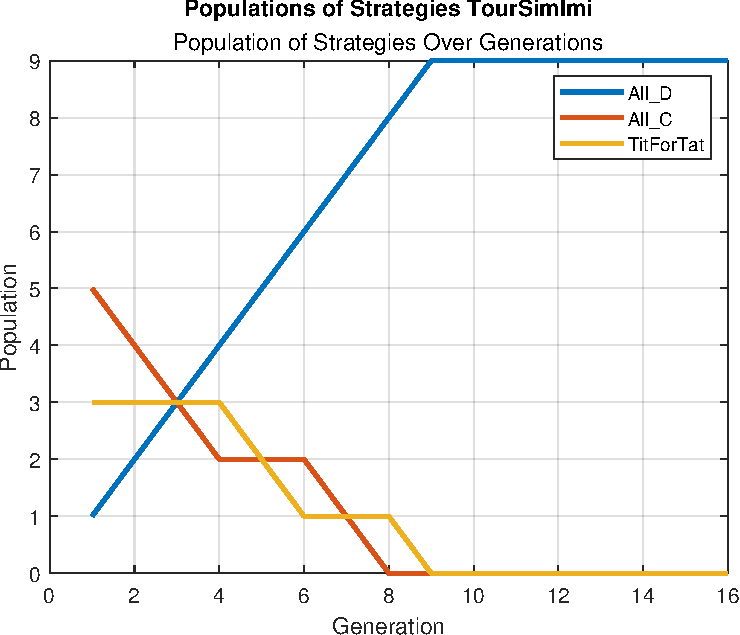
\includegraphics[width=.9\textwidth]{900.pdf}
			\caption{$\begin{bmatrix}9&0&0\end{bmatrix}$}
	      	\label{fig:900}
		\end{subfigure}%
		\begin{subfigure}{.5\textwidth}
			\centering
	      	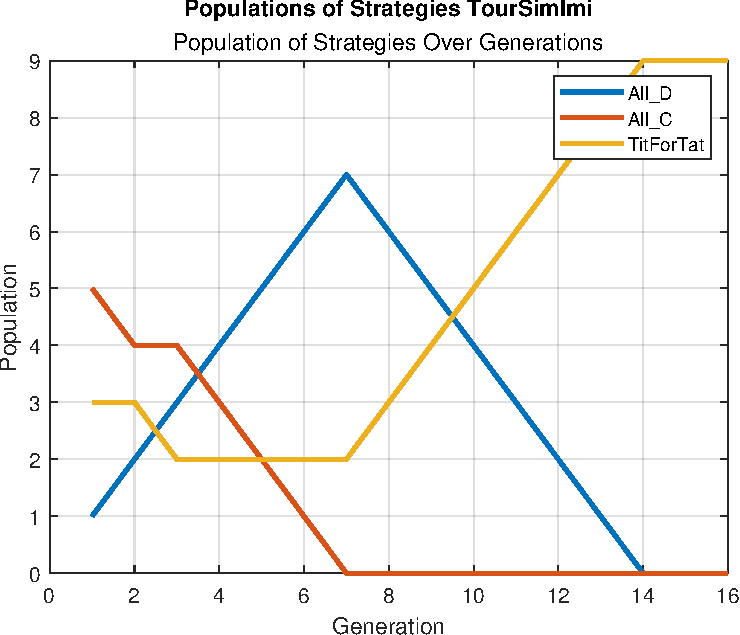
\includegraphics[width=0.90\textwidth]{009.pdf}
			\caption{$\begin{bmatrix}0&0&9\end{bmatrix}$}
	      	\label{fig:009}
		\end{subfigure}
		\caption{Absorbing States may differ even for the same Starting State}
		\label{fig:TourSimImi153}
	\end{figure}

\subsubsection{2η Προσομοίωση - Δοκιμή προεπιλεγμένης μεθόδου (Individual) για τον προσδιορισμό της καλύτερης στρατηγικής}
Στις δύο επόμενες προσομοιώσεις επιχειρείται να παρουσιαστεί η διαφορά στα αποτελέσματα που προκαλεί η διαφορετική μεθοδολογία επιλογής της καλύτερης στρατηγικής. Αρχικά (\ref{fig:TourTheImiIndividual}) παρουσιάζεται η μαρκοβιανή αλυσίδα που προκύπτει για αρχικό μείγμα στρατηγικών $\begin{bmatrix}1&4&5\end{bmatrix}$ και επιλογή μεθόδου ``Individual'', δηλαδή επιλογή της καλύτερης στατηγικής με σύγκριση των payoffs των στρατηγικών με παιχνίδια ένας εναντίον ενός για κάθε ζεύγος στρατηγικών.

Το αποτέλεσμα είναι αντίστοιχο αυτού της πρώτης προσομοίωσης \ref{fig:TourTheImi153}. Με λίγη παρατήρηση μπορούμε να οραματιστούμε μία νοητή καμπύλη μεταξύ των κορυφών των καταστάσεων $\begin{bmatrix}8&0&2\end{bmatrix}, \begin{bmatrix}6&1&3\end{bmatrix}, \begin{bmatrix}4&2&4\end{bmatrix}, \begin{bmatrix}2&3&5\end{bmatrix}$ η οποία χωρίζει τις λεκάνες απορροής των συμπαθών και των μη-συμπαθών στρατηγικών. Αν βρεθούμε σε κατάσταση κάτω από αυτή την καμπύλη θα καταλήξουμε στην απορροφητική κατάσταση επικράτησης της ``All\_D'', ενώ από κατάσταση πάνω από αυτή την καμπύλη θα καταλήξουμε σε μία από τις απορροφητικές καταστάσεις των συμπαθών στρατηγικών.
	\begin{figure}[h]
	      \centering
	      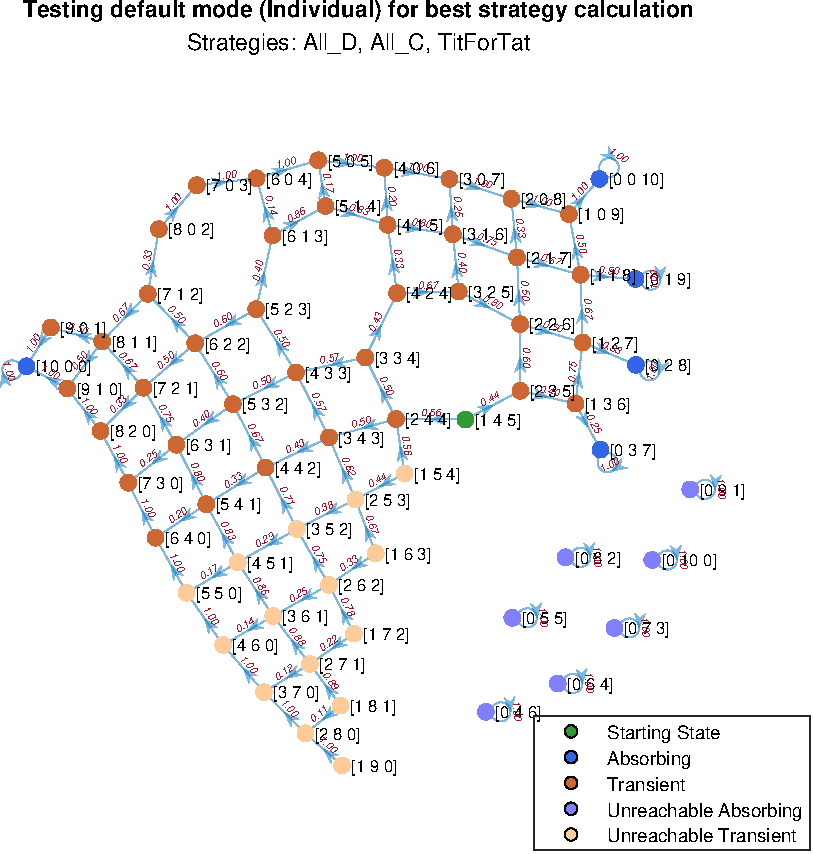
\includegraphics[width=0.95\textwidth]{Testing default mode (Individual) for best strategy calculation.pdf}
	      \caption{Testing default mode (``Individual'') for best strategy calculation with $POP0=\begin{bmatrix}1&4&5\end{bmatrix}$}
	      \label{fig:TourTheImiIndividual}
	\end{figure}
\subsubsection{3η Προσομοίωση - Δοκιμή μεθόδου ``Total'' για τον προσδιορισμό της καλύτερης στρατηγικής}
Στην τρίτη προσομοίωση (\ref{fig:TourTheImiTotal}) για ίδιο αρχικό μείγμα στρατηγικών $\begin{bmatrix}1&4&5\end{bmatrix}$ και επιλογή μεθόδου ``Total'', δηλαδή σύγκριση των payoffs των παικτών που προκύπτουν σε κάθε state από Axelrod με τους πληθυσμούς του state και επιλογή ως καλύτερη στρατηγική της στρατηγικής του παίκτη με το μεγαλύτερο συνολικό payoff.

Σε αντίθεση με την προηγούμενη προσομοίωση (\ref{fig:TourTheImiIndividual}) εδώ παρατηρούμε ότι το διάγραμμα είναι χωρισμένο σε τρεις ξεχωριστούς υπογράφους.
Ο πρώτος υπογράφος, αυτός που περιλαμβάνει την αρχική κατάσταση, είναι ο μόνος που περιλαμβάνει προσεγγίσιμη απορροφητική κατάσταση (την $\begin{bmatrix}0&0&10\end{bmatrix}$), η οποία είναι η επικράτηση της ``TitForTat''. Αυτό συμβαίνει διότι κατά την εύρεση της καλυτερης στρατηγικής στο mode ``Total'' οι συμπαθείς στρατηγικές συνεργάζονται μεταξύ τους και υπερνικούν λόγω του μεγαλύτερου πλήθους τους το προβάδισμα που δίνει η λιποταξία στην ``All\_D''
Ο δεύτερος υπογράφος είναι αυτός που περιλαμβάνει την απορροφητική κατάσταση που επικρατεί η ``All\_D'' ($\begin{bmatrix}10&0&0\end{bmatrix}$), η οποία όμως είναι μη προσπελάσιμη όπως και οι μεταβατικές καταστάσεις όλου του υπογράφου, για τον λόγο που περιγράφηκε παραπάνω.
Τέλος ο τρίτος υπογράφος είναι αυτός που περιλαμβάνει την απορροφητική κατάσταση που επικρατεί η ``All\_C'' ($\begin{bmatrix}0&10&0\end{bmatrix}$), η οποία είναι επίσης μη προσπελάσιμη όπως και οι μεταβατικές καταστάσεις όλου του υπογράφου, για τον λόγο που περιγράφηκε παραπάνω.

	\begin{figure}[h]
	      \centering
	      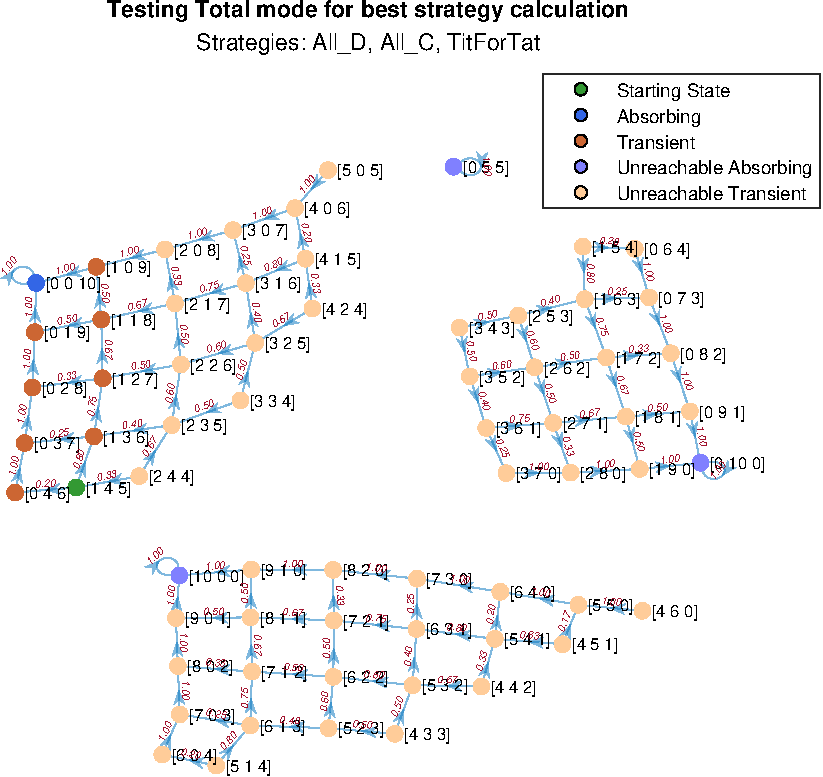
\includegraphics[width=0.95\textwidth]{Testing Total mode for best strategy calculation}
	      \caption{Testing ``Total'' mode for best strategy calculation with $POP0=\begin{bmatrix}1&4&5\end{bmatrix}$}
	      \label{fig:TourTheImiTotal}
	\end{figure}

\clearpage
\section{Σύγκριση Fitness vs Imitation Dynamics}
	\begin{figure}[h]
	      \centering
	      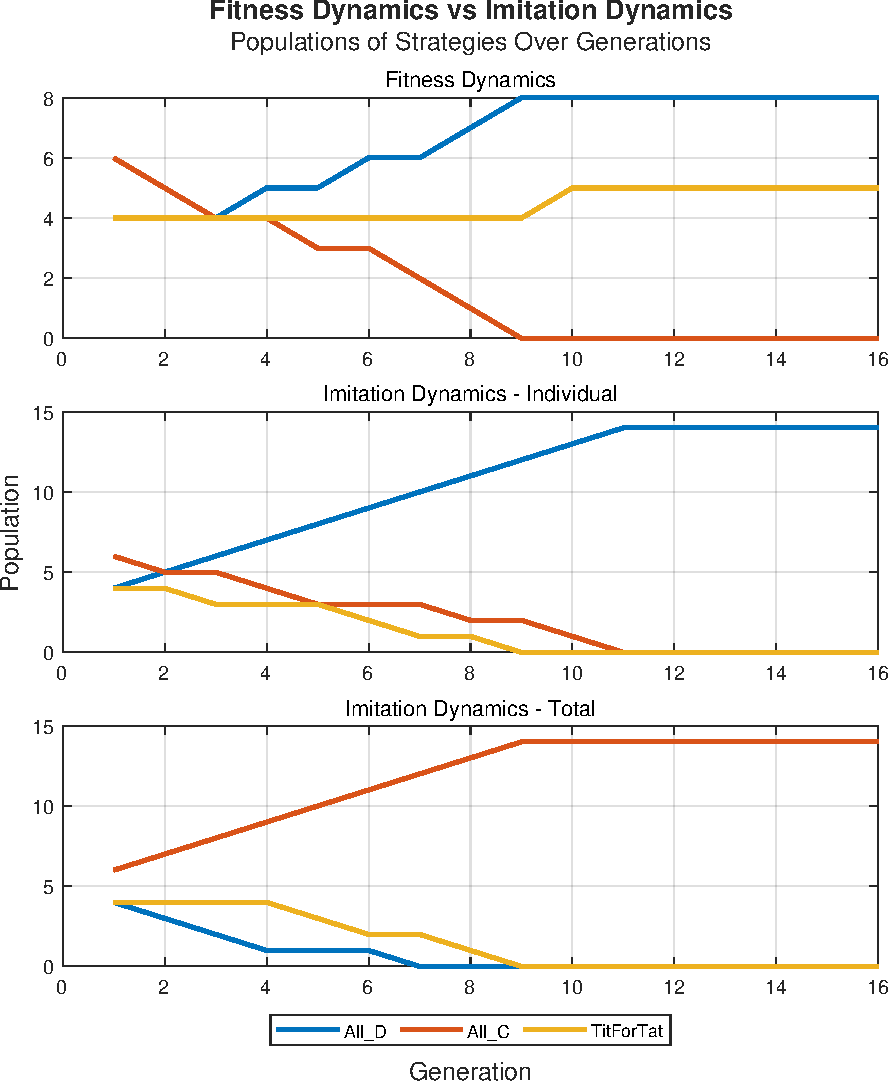
\includegraphics[width=0.9\textwidth]{Fitness Dynamics vs Imitation Dynamics.pdf}
	      \caption{Fitness Dynamics vs Imitation Dynamics $\begin{bmatrix}All\_D&All\_C&TitForTat\end{bmatrix}$ $POP0=\begin{bmatrix}4&6&4\end{bmatrix}$}
	      \label{fig:Fitness Dynamics vs Imitation Dynamics}
	\end{figure}
Στο Σχήμα \ref{fig:Fitness Dynamics vs Imitation Dynamics} γίνεται μία σύγκριση μεταξύ των αποτελεσμάτων των TourSimFit, TourSimImi με mode=''Individual'' και TourSimImi με mode=''Total'' για στρατηγικές $\begin{bmatrix}All\_D&All\_C&TitForTat\end{bmatrix}$ με $POP0=\begin{bmatrix}4&6&4\end{bmatrix}$.
Παρατηρούμε ότι η περίπτωση Fitness μοιάζει με την περίπτωση ``Individual'' mode, ωστόσο και μεταξύ των δύο σημειώνεται η σημαντική διαφορά ότι στα Imitation Dynamics επιβιώνει μόνο μία στρατηγική. Η περίπτωση του ``Total'' mode έχει παρόμοια εξέλιξη με το ``Individual'' mode αλλά παρατηρούμε ότι επιβιώνει διαφορετική στρατηγική, συγκεκριμένα η ``All\_C'', επειδή έχει αρχικό πληθυσμό μεγαλύτερο από τις άλλες στρατηγικές και άρα εκμεταλλεύεται καλύτερα την συμπαθή στρατηγική ``TitForTat'' μέσω της λειτουργίας του ``Total'' mode για εύρεση της βέλτιστης στρατηγικής.


\clearpage
\section{Τελικά Συμπεράσματα}
Από την παραπάνω ανάλυση των δύο εξελικτικών δυναμικών προκύπτουν τα παρακάτω συμπεράσματα:

\subsection*{Για τα Fitness Dynamics}
α) Οι Mathieu et al φαίνεται ότι χρησιμοποιούσαν απλό floor κατά τον υπολογισμό των νέων πληθυσμών μετά από κάθε γενιά, καθώς η τακτική αυτή δημιούργησε για εμάς τα κοντινότερα αποτελέσματα.

β) Σε πολλές περιπτώσεις ασταθών, γενικά, συμπεριφορών, τα διαγράμματα διαφοροποιούνται σε παρατηρήσιμο βαθμό ανάλογα με το αν χρησιμοποιείται η συνάρτηση TourTheFit ή η συνάρτηση TourSimFit με και χωρίς compensation. Αυτό οφείλεται στο ότι πολλές από τις περιπτώσεις των διαγραμμάτων που προκύπτουν είναι ιδιαίτερα ευαίσθητες και έτσι, ακόμα και μικρή μεταβολή στη λογική της δυναμικής, μπορεί να αλλάξει τα αποτελέσματα σημαντικά.

γ) Το διάγραμμα που προκύπτει εξαρτάται από τις αρχικές τιμές πληθυσμού, τις στρατηγικές που χρησιμοποιούνται και τον πίνακα απολαβής. Ακόμα και για 2 από αυτούς τους παράγοντες ίδιους, η μεταβολή ενός από αυτούς μπορεί να οδηγήσει σε δραστικά διαφορετικά αποτελέσματα (ακόμα και διαφορετική ταξινόμηση, όπως στην 5η προσομοίωση).

δ) Η ανάθεση των εναπομείναντων μελών του πληθυσμού τυχαία σύμφωνα με τη λογική του compensation φαίνεται να είναι καλή επιλογή, ειδικά σε σχέση με την απλότητά της, διότι δε μεταβάλλει σημαντικά τα αποτελέσματα (στρατηγικές που θεωρητικά πεθαίνουν, πεθαίνουν πραγματικά, γενικά το πού τείνουν οι πληθυσμοί δεν αλλάζει). Ανάλογα με την περίπτωση που εξετάζεται, μοιάζει περισσότερο είτε με την περίπτωση της TourTheFit είτε με την περίπτωση TourSimFit δίχως compensation.

ε) Σε γενικές γραμμές, η διακριτή φύση των προσομοιώσεων TourSimFit με ή χωρίς compensation, δημιουργεί σε βάθος χρόνου είτε επαναλαμβανόμενες ταλαντώσεις είτε σύγκλιση σε κάποιες τελικές τιμές πληθυσμού. Το χάος δεν μπορεί πραγματικά να επιτευχθεί, ακόμα και στην 6η προσομοίωση οι πληθυσμοί τελικά τείνουν στις τιμές που προβλέπει και η TourTheFit. Ωστόσο, αυτό δε μας αποτρέπει από το να δημιουργήσουμε τα ενδιαφέροντα αποτελέσματα που βλέπουμε και στο paper.

\subsection*{Για τα Imitation Dynamics}
α) Η επιλογή της ακριβής δυναμικής που ακολουθάται κατά τον υπολογισμό των πληθυσμών της επόμενης γενιάς είναι βασική για τα αποτελέσματα που προκύπτουν. Για παράδειγμα, η επιλογή K παικτών από τον συνολικό πληθυσμό ή K παικτών εκ των μη βέλτιστων, δημιουργούν πολύ διαφορετικά αποτελέσματα και θεωρητικά και στις προσομοιώσεις.

β) Οι περιπτώσεις υπολογισμού της βέλτιστης στρατηγικής με τη μέθοδο In\-di\-vi\-du\-al και Total οδηγούν επίσης σε δραστικά διαφορετικά αποτελέσματα για τη φύση των καταστάσεων που προκύπτουν, όπως φαίνεται στις προσομοιώσεις 2 και 3. Σε γενικές γραμμές, η μέθοδος Total δημιουργεί συνεκτικούς υπογράφους που έχουν ως τελικές καταστάσεις τις καταστάσεις επικράτησης μίας εκ των στρατηγικών, ενώ η μέθοδος Individual δημιουργεί έναν μεγαλύτερο υπογράφο που οδηγεί σε πολλές πιθανές τελικές καταστάσεις και μερικές απομονωμένες τελικές καταστάσεις. Ο όρος συνεκτικότητα χρησιμοποιείται εδώ λανθασμένα, καθώς πρόκειται για κατευθυνόμενους γράφους στους οποίους κατά κανόνα δεν υπάρχουν διαδρομές και προς τις δύο κατευθύνσεις, αλλά χρησιμοποιείται για τη χαλαρή επεξήγηση του φαινομένου.

γ) Λόγω του β), παρατηρούμε ότι η τελική κατάσταση δεν είναι πάντα βέβαιη γνωρίζοντας την αρχική, εφόσον επιλέγεται η μέθοδος Individual. Αυτό οφείλεται στο ότι η τυχαία ανάθεση ανά γενιά μπορεί να οδηγήσει διαφορετικές κάθε φορά στρατηγικές σε πλεονεκτική θέση την επόμενη γενιά, και άρα να υπάρχει μεταβλητότητα στα αποτελέσματα. Αντιθέτως, η μέθοδος Total είναι πλήρως ντετερμινιστική ως προς την αρχική και τελική κατάσταση, ενώ παρουσιάζει τυχαιότητα μόνο στο μονοπάτι που θα ακολουθηθεί μεταξύ των 2.

δ) Σε κάθε περίπτωση, οι πληθυσμοί που προκύπτουν από τη συνάρτηση Tour\-Sim\-Imi ακολουθούν κάποια σειρά μεταβολών που παρουσιάζεται στο διάγραμμα μετάβασης καταστάσεων της αντίστοιχης Tour\-The\-Imi και Analyze\-Markov\-Chain.
\clearpage
\listoffigures\addcontentsline{toc}{section}{List of Figures}
\end{document}